% This is samplepaper.tex, a sample chapter demonstrating the
% LLNCS macro package for Springer Computer Science proceedings;
% Version 2.21 of 2022/01/12
%
\documentclass[runningheads]{llncs}


% \usepackage[utf8]{inputenc}
% \usepackage[margin=0.8in]{geometry}




\usepackage{color}
\usepackage{amsmath}
%\usepackage{amssymb}
\usepackage{graphicx}
% \usepackage{amsthm}
\usepackage{stmaryrd}
\usepackage[all]{xy}
\usepackage{multirow}
\usepackage{paralist}
\usepackage{hhline}
\usepackage{bm}
\usepackage{longtable}
\usepackage{makecell}
\usepackage{mdframed}

\usepackage{wasysym}
\usepackage{extarrows}
\usepackage{tikz}

% add new commands for comments here
\newcommand{\yx}[1]{\textit{\color{blue}[YX] : #1}}
\newcommand{\gb}[1]{\textit{\color{green}[GB] : #1}}
\newcommand{\lz}[1]{\textit{\color{red}[LZ] : #1}}

\newcommand{\modify}[1]{{\color{red}#1}}

\usepackage{amssymb}
\usepackage{amsmath}
\usepackage{stmaryrd}
\usepackage{hyperref}

\usepackage{braket}
\usepackage{cleveref}

\usepackage{algorithm}
\usepackage{algpseudocode}


\usepackage{listings}
\usepackage[dvipsnames]{xcolor}


\lstdefinestyle{dirace}{
    columns=fullflexible,
    mathescape = true,
    sensitive=true,
    basicstyle=\ttfamily\small, % Set sans-serif font as basic font
    breaklines=true,
    backgroundcolor=\color{lightgray!50!white}, % Light gray background
    morekeywords=[1]{Def, Var, CheckEq, with},
    morekeywords=[2]{INDEX, OTYPE, REG, USET}, 
    keywordstyle=[1]\bfseries\color{NavyBlue},
    keywordstyle=[2]\bfseries\color{black}, 
    %  emph={self},
    % emphstyle=\bfseries\color{Rhodamine},
    morecomment=[l]{//},
    commentstyle=\itshape\color{black!50!white},
    string=[b]"
}

\usepackage{tikz}
\usetikzlibrary{shapes.geometric, arrows}
\usetikzlibrary{trees}
\tikzstyle{arrow} = [thick,->,>=stealth]



\newenvironment{ruletable}[1]
{
    \begin{longtable}{p{3cm} l}
    \caption{#1}\\
    \hline
    \textbf{Rule} & \textbf{Description} \\
    \hline
    \endfirsthead

    \hline
    \textbf{Rule} & \textbf{Description} \\
    \hline
    \endhead

    % \hline
    % \multicolumn{2}{r}{\textit{Continued on the next page}} \\
    \hline
    \endfoot

    \hline
    \endlastfoot
}
{
    \end{longtable}
}

% define C++ logo
\newcommand{\CC}{C\nolinebreak\hspace{-.05em}\raisebox{.4ex}{\tiny\bf +}\nolinebreak\hspace{-.10em}\raisebox{.4ex}{\tiny\bf +}}
\def\CC{{C\nolinebreak[4]\hspace{-.05em}\raisebox{.4ex}{\tiny\bf ++}}}

\def\>{\ensuremath{\rangle}}
\def\<{\ensuremath{\langle}}

\newcommand {\cH } {{\mathcal{H}}}
\newcommand {\bu } {{\mathbf{u}}}
\newcommand {\bv } {{\mathbf{v}}}
\newcommand {\bC } {{\mathbb{C}}}
\newcommand {\ghz } {{\mathrm{GHZ}}}
\newcommand {\cnot } {{\mathsf{CNOT}}}
\newcommand {\ccnot } {{\mathsf{CCNOT}}}
\newcommand {\swap } {{\mathsf{SWAP}}}
\renewcommand{\matrix}[1]{\begin{bmatrix}#1\end{bmatrix}}


%
\usepackage[T1]{fontenc}
% T1 fonts will be used to generate the final print and online PDFs,
% so please use T1 fonts in your manuscript whenever possible.
% Other font encondings may result in incorrect characters.
%
\usepackage{graphicx}
% Used for displaying a sample figure. If possible, figure files should
% be included in EPS format.
%
% If you use the hyperref package, please uncomment the following two lines
% to display URLs in blue roman font according to Springer's eBook style:
\usepackage{color}
\renewcommand\UrlFont{\color{blue}\rmfamily}
\urlstyle{rm}
%
\begin{document}
%
\title{D-Hammer: Efficient Equational Reasoning for Labelled Dirac Notation}
\author{}
\institute{}

%%%%%%%%%%%%%%%%%%%%%%%%%%%%%%%%%%%%%%%%%%%%%%%%%%%%%%%%%%%%%%%%%%%%%%%%
% %
% %\titlerunning{Abbreviated paper title}
% % If the paper title is too long for the running head, you can set
% % an abbreviated paper title here
% %
% \author{First Author\inst{1}\orcidID{0000-1111-2222-3333} \and
% Second Author\inst{2,3}\orcidID{1111-2222-3333-4444} \and
% Third Author\inst{3}\orcidID{2222--3333-4444-5555}}
% %
% \authorrunning{F. Author et al.}
% % First names are abbreviated in the running head.
% % If there are more than two authors, 'et al.' is used.
% %
% \institute{Princeton University, Princeton NJ 08544, USA \and
% Springer Heidelberg, Tiergartenstr. 17, 69121 Heidelberg, Germany
% \email{lncs@springer.com}\\
% \url{http://www.springer.com/gp/computer-science/lncs} \and
% ABC Institute, Rupert-Karls-University Heidelberg, Heidelberg, Germany\\
% \email{\{abc,lncs\}@uni-heidelberg.de}}
%%%%%%%%%%%%%%%%%%%%%%%%%%%%%%%%%%%%%%%%%%%%%%%%%%%%%%%%%%%%%%%%%%%%%%%%


%
\maketitle              % typeset the header of the contribution
%
\begin{abstract}
Labelled Dirac notation is a formalism commonly used by physicists to
represent many-body quantum systems and computer scientists to assert
properties of quantum programs. Labelled Dirac notation is supported
by a rich equational theory for proving equality between expressions
of the language. These proofs are typically carried on pen-and-paper,
and can be exceedingly long and error-prone. We introduce D-Hammer,
the first tool to supported automated equational proof for labelled
Dirac notation. The salient features of D-Hammer are: an expressive,
higher-order, dependently-typed language for labelled Dirac notation;
an efficient algorithm to normalize expressions (modulo associativity
and commutativity); and an optimized \CC\ implementation. We evaluate
the implementation on representative examples from plain and labelled
Dirac notation. In the case of plain Dirac notation, we show that our
implementation significantly outperforms DiracDec (Xu et al, POPL'25).
  


% \keywords{First keyword  \and Second keyword \and Another keyword.}
\end{abstract}
%
%
%



%%%%%%%%%%%%%%%%
\newcommand*{\sem}[1]{{\llbracket #1 \rrbracket}}
\newcommand{\DiracDec}{\textsf{DiracDec}}

\newcommand{\reduce}{\triangleright}

\newcommand{\Sort}{\mathsf{Sort}}
\newcommand{\WF}{\mathcal{WF}}

\newcommand{\Index}{\mathsf{Index}}
\newcommand{\Type}{\mathsf{Type}}
\newcommand{\Basis}{\mathsf{Basis}}

\newcommand{\SType}{\mathcal{S}}
\newcommand{\KType}{\mathcal{K}}
\newcommand{\BType}{\mathcal{B}}
\newcommand{\OType}{\mathcal{O}}
\newcommand{\SET}{\mathsf{Set}}

\newcommand{\ZEROK}{\mathbf{0}_\mathcal{K}}
\newcommand{\ZEROB}{\mathbf{0}_\mathcal{B}}
\newcommand{\ZEROO}{\mathbf{0}_\mathcal{O}}

\newcommand{\PAIR}{\mathsf{PAIR}}

\newcommand{\ZERO}{\mathsf{0}}
\newcommand{\ONE}{\mathsf{1}}
\newcommand{\ADDS}{\mathsf{ADDS}}
\newcommand{\ADD}{\mathsf{ADD}}
\newcommand{\MULS}{\mathsf{MULS}}
\newcommand{\MUL}{\mathsf{MUL}}
\newcommand{\CONJ}{\mathsf{CONJ}}
\newcommand{\CJG}{\mathsf{CJG}}
\newcommand{\ADJ}{\mathsf{ADJ}}
\newcommand{\DELTA}{\mathsf{DELTA}}
\newcommand{\DOT}{\mathsf{DOT}}
\newcommand{\SCR}{\mathsf{SCR}}
\newcommand{\TSR}{\mathsf{TSR}}
\newcommand{\KET}{\mathsf{KET}}
\newcommand{\BRA}{\mathsf{BRA}}
\newcommand{\ONEO}{\mathbf{1}_\mathcal{O}}
\newcommand{\OUTER}{\mathsf{OUTER}}
\newcommand{\MULK}{\mathsf{MULK}}
\newcommand{\MULB}{\mathsf{MULB}}
\newcommand{\MULO}{\mathsf{MULO}}



\newcommand{\var}{\mathsf{var}}
\newcommand{\reg}{\mathsf{Reg}}
\newcommand{\DType}{\mathcal{D}}
\newcommand{\cR}{\mathcal{R}}
\newcommand{\cN}{\mathcal{N}}
\newcommand{\tD}{\tilde{D}}
\newcommand{\te}{\tilde{e}}
\newcommand{\tT}{\tilde{T}}
\newcommand{\tADD}{\widetilde{ADD}}
\newcommand{\bU}{\mathbf{U}}
\newcommand{\<}{\langle}
\newcommand{\simp}{\mathsf{Simp}}
\newcommand{\List}{\mathsf{list}}
\renewcommand{\>}{\rangle}

%%%%%%%%%%%%%%%%%%%%%%%%%%%



\section{Introduction}


Dirac notation~\cite{dirac1939new}, a.k.a.\, bra-ket notation, is a
mathematical formalism for representing quantum states using linear
algebra notation: for instance, Dirac notation uses the linear
combination \( a\ket{\psi} + b\ket{\phi} \) to represent the
superposition of the two quantum states \( \ket{\psi} \) and
\( \ket{\phi} \). Another essential ingredient of Dirac notation
is the tensor product $\otimes$, which is used to describe composite
states: for instance, Dirac notation uses the tensor expression
\( \ket{\psi} \otimes \ket{\phi} \) to denote the composition of
the two quantum states \( \ket{\psi} \) and \( \ket{\phi} \). It is
also common to use a variant of Dirac notation, called labelled Dirac
notation, to describe composite quantum states. In labelled Dirac
notation, bras and kets are tagged with labels that identify the
subsystems on which they operate. For instance, the labelled tensor
expression
\( \ket{\psi}_{S'} \otimes \ket{\phi}_{S} \)
states that $\ket{\psi}_S$ and $\ket{\psi}_{S'}$ describe two quantum
states over some subsystem $S$ and $S'$ respectively. By considering
the relationship between $S$ and $S'$, one can obtain identities for
free, e.g.\, 
%
$$\ket{\phi}_S \otimes \ket{\psi}_{T} = \ket{\psi}_{T} \otimes \ket{\phi}_S
\mbox{if}~S\cap S'=\emptyset$$
%
In turn, commutativity of the tensor product ensures that one can
reason locally about quantum systems, and contributes to making
labelled Dirac notation a convenient, compositional formalism to
reason about quantum states---in a way that is similar to the way
bunched logics support compositional reasoning about mutable states.

Labelled Dirac notation is also commonly used to express assertions
about quantum programs. Specifically, many quantum Hoare logics use
labelled Dirac notation to express program assertions~\cite{DBLP:conf/lics/ZhouBHYY21,Zhou2023}. These logics also use
implicitly equational reasoning between labelled Dirac expressions, to
glue applications of proof rules---similar to the use of the rule of
consequence in the setting of classical program. Therefore, it is
essential for the verification of quantum programs to have automated
means of proving equality of two complex expressions based on labelled
Dirac notation.


\subsubsection*{Contributions}
This paper presents an automated tool, called D-Hammer, for reasoning
about labelled Dirac notation. D-Hammer uses a rich, dependently typed
language, to formalize labelled Dirac notation, and supports common
idioms used to describe quantum systems, including big operators of
the form $\sum_{i\in I} a_i \ket{\phi_i}_S$ to represent indexed
superpositions of states. The semantics of typable expressions is
given in terms of Hilbert spaces, tailored to interpreting tensor
product as an AC symbol. We leverage this interpretation to define a
rich equational theory for labelled Dirac notation, and prove its
soundness with respect to our denotational semantics. Finally, we
define an efficient normalization procedure to prove equivalence of
two expressions. We then evaluate our procedure with respect to
examples from the literature. Our evaluation covers examples based on
(vanilla, unlabelled) Dirac notation, as well as examples based on
labelled Dirac notation. The main conclusions are that our approach
outperforms prior work by~\cite{diracdec} and is able to prove complex
examples of reasoning with labelled Dirac notation from the
literature, including examples from prior work on quantum separation
logic~\cite{DBLP:conf/lics/ZhouBHYY21}.



%% In 1939, Dirac introduced his notation for quantum mechanics~\cite{dirac1939new}, designed to represent linear algebraic formulas in a compact and convenient form. For example, the expression \( a\ket{\psi} + b\ket{\phi} \) represents the superposition of two quantum states, \( \ket{\psi} \) and \( \ket{\phi} \). Today, Dirac notation is widely accepted as the standard language in quantum computation and quantum information. Its reasoning forms the foundation of research and applications, much like boolean and integer logic do in classical computer science.

%% In quantum algorithm formalizations and quantum programming languages, Dirac notation is frequently used in equational proofs, which are critical, repetitive, and often time-intensive. These notations also play a key role in defining program states, operations, and assertions in quantum programming languages. To automate the verification of these programs, we need tools that can simplify and check the equivalence of preconditions. However, unlike the well-established SAT and SMT solvers for classical logic, a practical solver for Dirac notation equivalence remains an unmet need, creating a barrier for progress in several fields.

%% Recently, Xu et al.~\cite{diracdec} proposed a theory for deciding the equivalence of Dirac notation, alongside a prototype implementation in Mathematica called DiracDec. They demonstrated that the equivalence of basic Dirac notation is decidable. Their algorithm, based on a pure term rewriting system, has been proven to be confluent and terminating. Despite this, there remains a gap between DiracDec and a practical solver for Dirac notation equivalence.

%% One challenge is the efficiency of the algorithm when dealing with equivalences beyond the scope of term rewriting. DiracDec decides the entire equational theory by rewriting modulo \( E \), where \( E \) represents a set of axioms that cannot be decided by normalization alone, such as the associativity and commutativity (AC) of certain function symbols. DiracDec uses a direct but inefficient algorithm to decide these axioms, which searches through all possible permutations and exhibits factorial complexity. This inefficiency becomes particularly evident in "computational examples" containing many AC symbols, which are time-consuming to process.

%% Usability is another area where DiracDec falls short. It does not support labelled Dirac notation, which uses registers to denote subsystems and express states locally. Additionally, DiracDec's typing system only does not provide context for variable typing assumptions or the definition of symbols, which are required in practical scenarios. To avoid type checking during term rewriting, DiracDec separates symbols (e.g., multiplication) for different types, leading to unnecessary complexity. Moreover, integrating the Mathematica implementation into other projects as a solver is challenging.

%% The system design of DiracDec reflects a trade-off between simplicity and efficiency. While the simplicity of term rewriting allows for strong theoretical results, it limits optimization opportunities. Building on DiracDec, this work aims to develop a practical solver. We transform the term rewriting system into a hybrid algorithm, overcoming the challenges mentioned above. Our main technical contributions are:
%% \begin{itemize}
%%     \item An efficient algorithm for deciding the equational theories in \( E \), based on equivalence checking through normalization, with the normal form for \( E \) being obtained via sorting.
%%     \item Support for constant register labels, and reducing the equivalence decision of labelled Dirac notation to the unlabelled case.
%%     \item A more user-friendly \CC\ solver, D-Hammer, featuring an abstract language and typing system. We also support the definition of symbols (e.g., transpose and trace) using function syntax.
%% \end{itemize}

%% We evaluated D-Hammer against the DiracDec benchmark and new examples involving labelled Dirac notation. The results show significant improvements in both decidability and efficiency compared to DiracDec.

%% % D-Hammer successfully decides all the examples that are expressable in its language, including those failed by DiracDec because of complexity or insufficient decision power.


\section{Motivation and Preliminaries}
\subsection{Standard Dirac Notation}

Dirac notation, also known as bra-ket notation, provides an intuitive
and concise mathematical framework for describing quantum states and
operations in quantum mechanics.  We write $\cH$ for a Hilbert space,
i.e., a vector space equipped with an standard inner product
$\langle\bu,\bv\rangle \in \bC$ for $\bu,\bv\in\cH$.  Dirac notation
consists of the following components that reflect the basic postulates
of quantum mechanics:
\begin{itemize}
  \item Ket $|u\rangle$ is a column vector that denotes a quantum state $\bu$ in the state Hilbert space $\cH$. For example, the computational bases of qubit system are commonly written as $|0\rangle = \matrix{1 \\ 0}$ and $|1\rangle = \matrix{0 \\ 1}$.
  \item Bra $\langle u|$ is a row vector, the conjugate transpose of $|u\rangle$, that denotes the dual state of $|u\rangle$. 
  %It is alternative to interpret as a linear mapping from $\cH$ to $\bC$ defined as $\langle u| : |v\rangle \mapsto \langle \bu,\bv\rangle$. It is the conjugate transpose of $|u\rangle$.
  For example, $\langle 0| = \matrix{1 & 0}$ and $\langle 1| = \matrix{0 & 1}$.
  \item Inner product $\langle u|v\rangle \triangleq \langle \bu,\bv\rangle$ which indicates the probability amplitude for $|u\rangle$ to collapse into $|v\rangle$. 
  By convention, it is computed by matrix multiplication of two states, e.g., 
  $\langle 0|1\rangle = \matrix{1 & 0} \matrix{0 \\ 1} = 0.$
  \item Outer product $|u\rangle\langle v| \triangleq |w\rangle \mapsto (\langle v|w\rangle) |u\rangle$. Any linear map, such as unitary tranformation, measurement operator, etc, can be decomposed as the sum of outer products. It is also computed by matrix multiplication, e.g., 
  $|1\rangle\langle 0| = \matrix{0 \\ 1} \matrix{1 & 0}  = \matrix{0 & 0 \\ 1 & 0}.$
  \item Tensor product $|u\rangle\otimes|v\rangle$ (or simply $|u\rangle|v\rangle$ or $|uv\rangle$), $\langle u|\otimes\langle v|$ (or simply $\langle u|\langle v|$ or $\langle uv|$) for describing the state, dual state and linear map of composite systems respectively. It is computed by the the Kronecker product of matrices, e.g., $\langle 0|\langle 1| = {\color{blue}\matrix{1 & 0}}\otimes {\color{red}\matrix{1 & 0}} = \matrix{({\color{blue}1}*{\color{red}1}) & ({\color{blue}1}*{\color{red}0}) & ({\color{blue}0}*{\color{red}1}) & ({\color{blue}0}*{\color{red}0})} = \matrix{1&0&0&0}$.
\end{itemize}

\subsection{Labelled Dirac Notation and Motivating Example}
Labelled Dirac notation is a generalization of Dirac notation for
describing multi-body quantum systems. The need for labelled Dirac
notation is motivated by the following example:

% \begin{figure}[t]
% \begin{quantikz}
%   & \gate{X} & \ctrl{1} & \\
%   & & \targ{} &
%   \end{quantikz}
%   =\begin{quantikz}
%   & \ctrl{1} & \gate{X} & \\
%   & \targ{} & \gate{X} &
%   \end{quantikz}
%   \end{figure}


\begin{example}
  \label{example1}
  Let $p,q,r$ be three qubits and initially in the (unnormalized)
  $\ghz$ state $|\ghz\rangle \triangleq |000\rangle+|111\rangle$.
  Applying the 3-qubit Toffoli gate ($\ccnot$) with control qubits
  $p,r$ and target qubit $q$ to GHZ is equivalent to applying 2-qubit
  $\cnot$ gate with control qubit $r$ or $p$ and target qubit $q$.
  Using Dirac notation, the identity is written as:
\begin{align*}
  \ccnot|\ghz\rangle &= (I\otimes \cnot)|\ghz\rangle \\
  &= (\Swap\otimes I)(I\otimes \cnot)(\Swap\otimes I)|\ghz\rangle
\end{align*}
which might be illustrated by the following circuit models.
\begin{figure}[h]
  % \begin{minipage}{0.48\linewidth}
      \centering
      \vspace{-0.5cm}
      \begin{quantikz}[column sep=0.1em, row sep=0em]
      \lstick{$p\qquad\qquad $} & \lstick{} &[0.2cm] & \ctrl{1} & [0.2cm] &  \quad \ \ \;\! \quad\qquad\quad & 
      &[0.2cm] & & [0.2cm] & \quad \ \ \;\! \quad\qquad\quad & 
      &[0.2cm] & \gate[2,swap,style={dashed}]{} & [0.2cm] & [0.2cm]\gate[2,swap,style={dashed}]{} & [0.2cm] & \\[-0.1cm]
      \lstick{$r\qquad\qquad $} & \lstick{$|\ghz\>$} & & \ctrl{1} & & \quad = \quad\qquad\quad & \lstick{$|\ghz\>$} 
      & & \ctrl{1} & & \quad = \quad\qquad\quad & \lstick{$|\ghz\>$}
      & & & \ctrl{1} & & & \\
      \lstick{$q\qquad\qquad $} & \lstick{} & & \targ{} & & \quad \ \ \;\! \quad\qquad\quad & 
      & & \targ{} & & \quad \ \ \;\! \quad\qquad\quad &
      & & & \targ{} & & & \\
      \end{quantikz}
      \vspace{-0.5cm}
      % \vspace{-0.7em}
      % \caption{Circuit computing the last bit of $a+(011)_2$.}
      % \label{fig:addition}
  %  \end{minipage}
  \end{figure}
Formalizing the statement in Dirac notation requires the following
steps: 1. Arrange qubits in the conventional order, here we choose
$p,r,q$ to simplify the representation of $\ccnot$; 2. Lift the local
operation $\cnot$ to the global system. For $\cnot$ acting on $r,q$ is
easier, since $r,q$ consistent with the chosen order, and we only need
to tensoring it by an identity operator $I$ on $p$, i.e., $(I\otimes
\cnot)$.  For $\cnot$ acting on $p,q$, realize that $p,q$ is not
adjacent in the chosen order, we additionally need to use $\Swap$ to
temporarily exchange the qubits $p$ and $r$, i.e., globally, the
$(\Swap\otimes I)$ before and after $(I\otimes \cnot)$ (lifting of
$\cnot$ on $r,q$).



Roughly speaking, encoding in standard Dirac notation needs to
tensoring identity operators and employing additional $\Swap$ gates
since generally the conventional order cannot guarantee 1. the order
of all local operations is consistent with it, 2. the local operations
involve only adjacent qubits in the conventional order.
\end{example}
To address the limitations of Dirac notations, physicists routinely
use labels (or subscripts) to indicate the systems on which quantum
states or operations are applied, thereby avoiding unnecessary lifting
and swap gates. For example, rewriting the above example using labels
yields:
\begin{align*}
  \ccnot_{prq}|\ghz\rangle_{pqr} = 
  \cnot_{rq}|\ghz\rangle_{pqr}
  = \cnot_{pq}|\ghz\rangle_{pqr}
\end{align*}
This formalization avoids determining and maintaining the conventional
order of qubits, nor lifting using additional $I$ and $\Swap$s. In
this setting, the tensor products become an associative and
commutative (AC) symbol, so we can rearrange qubits as needed to
perform calculations. For our example, we can perform the calculation as
follows:
\begin{align*}
  &\ccnot_{prq}|\ghz\rangle_{pqr}
  = (\ccnot|000\rangle + \ccnot|111\rangle)_{prq}
  = (|000\rangle + |110\rangle)_{prq}\\
  &\cnot_{rq}|\ghz\rangle_{pqr}
  = (\cnot|00\rangle)_{rq}|0\rangle_p + (\cnot|11\rangle)_{rq}|1\rangle_p
  =(|000\rangle + |101\rangle)_{rqp}\\
  &\cnot_{pq}|\ghz\rangle_{pqr}
  = (\cnot|00\rangle)_{pq}|0\rangle_r + (\cnot|11\rangle)_{pq}|1\rangle_r
  = (|000\rangle + |101\rangle)_{pqr}
\end{align*}
where the RHS of each line are equivalent.  In addition, labelled
Dirac notation can conveniently describe local measurements, partial
traces (the state or evolution of subsystems in multi-body systems),
and partial inner products (the representation of partial traces in
pure states), which are sufficient to handle the mathematical formulas
of quantum mechanics in multi-body systems.

Labelled Dirac notation is not only ubiquitous in the description of multi-body systems, but also plays an important role in program logics. Just as in classical program logic, variable names are used to construct logical formulas instead of describing them as global memory functions, in quantum program logic, variable names are used to label the subsystems on which quantum gates act, rather than lifting them to the global system. Indeed, the latter would cause exponential length of the formula w.r.t the number of variables, as discussed in [cite].

The next sections introduce the formal language, labelled Dirac notation and the systematical way to reduce labels and prove equalities. 
For this purpose, we use the following motivating example as the main role in our explanations.
Instead of GHZ states, it is a similar but simpler example on Bell states:
\begin{example}
    \label{ex: motivating}
    Let \( q \) and \( r \) represent two quantum systems in the Hilbert space \( \mathcal{H}_T \). Let \( M \) be a quantum operation acting on \( \mathcal{H}_T \), and let \( \ket{\Phi} = \sum_{i \in T} \ket{i} \otimes \ket{i} \) be the maximally entangled state. Then, it holds that
    \[
    M_q \ket{\Phi}_{(q, r)} = M_r^T \ket{\Phi}_{(q, r)}.
    \]
\end{example}
Following the introduction on labels, we can consider the global system $(q,r)$ and transform the equation above into the plain Dirac notation:
\begin{align}
    (M \otimes I) \ket{\Phi} = (I \otimes M^T) \ket{\Phi}.
    \label{eq: motivating plain}
\end{align}
Together with corresponding explanations for this example, we show how an automated system is built and used to solve equalities likewise.

% We will use the following
% generalization of Example \ref{example1} as motivating example:
% \begin{example}[Apply multiplexer to $\ghz$ state]
%   \label{ex: motivating}
%   Let $p,q,r$ be three quantum systems with the same Hilbert space \( \mathcal{H}_T \) (i.e., with computational bases $\{|i\>\}_{i\in T}$) and GHZ state $|\ghz\> = \sum_i|iii\>\<iii|$. Consider the linear operator sets $U_{ij}$ and the corresponding multiplexers $M\triangleq \sum_{ij}|ij\>\<ij|\otimes U_{ij}$ and $N\triangleq \sum_i|i\>\<i|\otimes U_{ii}$. We have:
%   $$M_{prq}|\ghz\>_{prq} = N_{rq}|\ghz\>_{pqr} = N_{pq}|\ghz\>_{pqr}.$$
% \end{example}

% An interesting property of quantum mechanics is that for two maximally entangled states, applying a quantum operator \( M \) to one subsystem is equivalent to applying \( M^T \) (the transpose of \( M \)) to the other subsystem. This relationship holds regardless of the spatial separation between the two systems, and it can be expressed as an equation in labelled Dirac notation.
% \begin{example}
%     \label{ex: motivating}
%     Let \( q \) and \( r \) represent two quantum systems in the Hilbert space \( \mathcal{H}_T \). Let \( M \) be a quantum operation acting on \( \mathcal{H}_T \), and let \( \ket{\Phi} = \sum_{i \in T} \ket{i} \otimes \ket{i} \) be the maximally entangled state. Then, we have the following equation:
%     \[
%     M_q \ket{\Phi}_{(q, r)} = M_r^T \ket{\Phi}_{(q, r)}.
%     \]
% \end{example}

% A little explanation on the notation and terms.
% Quantum states are represented as vectors in complex Hilbert spaces, and operations on these states are described by linear transformations, or operators. Dirac notation uses the ket \( \ket{i} \) and the bra \( \bra{i} \) to denote basis vectors in a Hilbert space and its dual space, respectively. These symbols can be composed together in various ways to form more complex expressions.
% For example, $M \ket{i}$ represents the operator-vector multiplication, and the tensor product \(\ket{i}\otimes\ket{i}\) describes the product state on multiple quantum systems.



% In this equation, \( q \) and \( r \) are labels denoting the respective subsystems in the Dirac notation. $M_q$ means that the operation $M$ is applied on system $q$, and $\ket{\Phi}_{(q, r)}$ denotes the quantum state $\ket{\Phi}$ on the (ordered) composed system $(q, r)$.
% To reason about their equivalence, we can remove the labels by extending them to the global system $(q, r)$:
% \begin{align}
%     (M \otimes I) \ket{\Phi} = (I \otimes M^T) \ket{\Phi}.
%     \label{eq: motivating unlabelled}
% \end{align}
% Here the identity operator $I$ are inserted in suitable positions to extend the operator $M$, a special case of extending to the global system called cylinder extension.

% \subsubsection{Universal Algebra}
% We use universal algebra and equational logic to formally represent Dirac notation and the reasoning procedure. A universal algebra defines a signature of function symbols, with terms constructed from constants, variables, and function applications. 
% Other basic concepts like substitution of variables or pattern matching are also defined.
% In our case of Dirac notation, the signature consists of constructors and operations like $\ket{i}$ or $A \otimes B$.
% The reasoning process is guided by equational logic, which defines an equivalence relation that is compatible with substitution and term construction. This relation formalizes the intuitive concept of equivalence in algebra.




\section{Language, Typing and Semantics}
The first step is to formalize the language for Dirac notation. In DiracDec, the language has a concrete design, where the same syntax for different types corresponds to distinct symbols. Our goal is to transition from this concrete design to a more abstract one, which aligns more closely with the conventional Dirac notation we use and simplifies the term rewriting system.

To achieve this, we organize our language into three layers: the index, the type, and the term. Terms represent concrete instances such as kets, bras, and operators, which will be typed and checked. The index represents classical data types and appears in type expressions to differentiate between various Hilbert spaces and sets.

\begin{definition}[Index Syntax]
    The syntax for type indices is:
    \begin{align*}
        \sigma ::=\ & x \mid \sigma_1 \times \sigma_2.
    \end{align*}
\end{definition}
Here, \( x \) is a variable, and \( \sigma_1 \times \sigma_2 \) represents the product type for tensor product spaces or Cartesian product sets.

\begin{definition}[Type Syntax]
    The syntax for Dirac notation types is:
    \begin{align*}
        T ::=\ & \Basis(\sigma) \mid \SType \mid \KType(\sigma) \mid \BType(\sigma) \mid \OType(\sigma_1, \sigma_2) \mid T_1 \to T_2 \mid \forall x.T \mid \SET(\sigma).
    \end{align*}
\end{definition}
\( \Basis(\sigma) \) denotes the type for basis elements in the index \( \sigma \).
\( \SType \) represents scalars, while \( \KType(\sigma) \) and \( \BType(\sigma) \) refer to ket and bra types in the Hilbert space \( \sigma \), respectively.
\( \OType(\sigma_1, \sigma_2) \) represents linear operators with \( \sigma_2 \) as the domain and \( \sigma_1 \) as the codomain.
\( \SET(\sigma) \) refers to the type of subsets of \( \sigma \), used to denote the values of bound variables in summations.
The remaining two constructs define function types: \( T_1 \to T_2 \) represents normal functions that take a \( T_1 \)-type argument and return a \( T_2 \)-type term, while \( \forall x. T \) represents index functions that take an index argument \( x \) and produce a \( T \)-type term, which may depend on \( x \).
Index functions are essential for defining polymorphic transformations across Hilbert spaces.


\begin{definition}[Term Syntax]
    The syntax for Dirac notation terms is:
    \begin{align*}
        e ::=\ & x \mid \lambda x : T.e \mid \mu x.e \mid e_1\ e_2 \mid (e_1, e_2) \\
        & |\ 0 \mid 1 \mid \ADDS(e_1, \cdots, e_n) \mid e_1 \times \cdots \times e_n \mid e^* \mid \delta_{e_1, e_2} \mid \DOT(e_1, e_2) \\
        & |\ \ZEROK(\sigma) \mid \ZEROB(\sigma) \mid \ZEROO(\sigma_1, \sigma_2) \mid \ONEO(\sigma) \\
        & |\ \ket{e} \mid \bra{t} \mid e^\dagger \mid e_1.e_2 \mid \ADD(e_1, \cdots, e_n) \mid e_1 \otimes e_2 \\
        & |\ \MULK(e_1, e_2) \mid \MULB(e_1, e_2) \mid \OUTER(e_1, e_2) \mid \MULO(e_1, e_2) \\
        & |\ \mathbf{U}(\sigma) \mid e_1 \star e_2 \mid \sum_{e_1} e_2.
    \end{align*}
\end{definition}
The terms above are explained in order:
\( \lambda x : T.e \) represents the abstraction for normal functions, and \( \mu x.e \) represents the abstraction for index functions.
\( e_1\ e_2 \) denotes function application.
\( (e_1, e_2) \) is the basis pair for product types.
The constants \( 0 \), \( 1 \), \( \ADDS \), \( e_1 \times \cdots \times e_n \), and \( e^* \) are symbols for scalars.
The next line includes constant symbols for kets, bras, and operators.
\( \ket{e} \) is a ket, \( \bra{t} \) is a bra, and \( e^\dagger \) denotes the conjugate transpose of \( e \).
\( e_1.e_2 \) represents scaling the term \( e_2 \) by scalar \( e_1 \).
\( \mathbf{U}(\sigma) \) denotes the universal set with index \( \sigma \).
\( e_1 \star e_2 \) represents the Cartesian product of \( e_1 \) and \( e_2 \).
\( \sum_{e_1} e_2 \) is the big operator sum, modeled by folding the function \( e_2 \) over the value set \( e_1 \). Typically, the sum's body is given by an abstraction. For convenience, we also use the notation \( \sum_{x \in s} X \) to represent \( \sum_{s} \lambda x : T . X \).
Additionally, \( \ADDS \) and \( \ADD \) are distinct AC symbols: \( \ADDS \) is used for scalar addition and \( \ADD \) for linear algebra addition.
There are five kinds of linear algebraic multiplications among kets, bras, and operators. These are encoded using five different symbols: \( \DOT \), \( \MULK \), \( \MULB \), \( \OUTER \), and \( \MULO \).

Compared to DiracDec, the symbols for addition, adjoint, scaling, and tensor products have been consolidated.
The multiplications are still kept separate due to their differing properties.
These operations are denoted as \( B \cdot K \), \( K_1 \cdot K_2 \), \( B_1 \cdot B_2 \), \( K \cdot B \), and \( O_1 \cdot O_2 \), respectively.




\subsection{Typing System}


The typing system is responsible for classifying terms within a proof system, using a context that specifies the types of variables and definitions. The context is divided into two components: the environment \( E \), which includes definitions and assumptions, and the context \( \Gamma \), which tracks bound variables. Both \( E \) and \( \Gamma \) consist of sequences of assumptions \( x : T \) or definitions \( x := t : T \).
\begin{definition}[Environment and Context]
    The syntax for \( E \) and \( \Gamma \) is:
    \begin{align*}
        E ::= &\ [] \mid E; x : \Index \mid E; x : T \mid E; x := t : T. \\
        \Gamma ::= &\ [] \mid \Gamma; x : \Index \mid \Gamma; x : T.
    \end{align*}
\end{definition}
Definitions refer to symbols that can be expanded or unfolded, and typically represent abstract concepts, such as transpose or trace in Dirac notation. Assumptions, on the other hand, define the types of variables, and variable assumptions are implicitly universally quantified in the case of equational proofs.

Type checking in our language involves maintaining a well-formed environment and context \( E[\Gamma] \). We say an expression \( t \) has type \( X \) in context \( E[\Gamma] \) if the typing judgment \( E[\Gamma] \vdash t : X \) can be proven through the rules in~\Cref{sec: full typing rules}. The well-formedness of the context \( \WF(E)[\Gamma] \) is built incrementally:
\[
    \frac{}{\WF([])[]}
    \qquad
    \frac{\WF(E)[] \qquad x \notin E}{\WF(E; x : \Index)[]}
    \qquad
    \frac{E[]\vdash t:T \qquad x \notin E}{\WF(E; x := t:T)[]}.
\]
Starting with an empty context, new index symbols can be introduced, and symbols with checked types can be defined. Typing judgments are then made inductively using the information from \( E[\Gamma] \). For instance, the rule \( x : \Index \in E[\Gamma] \) holds if \( E \) or \( \Gamma \) contains an assumption for \( x \).
And \(\KType(\sigma)\) is a valid type for kets, if the argument $\sigma$ is typed as an index.
\begin{gather*}
    \frac{\WF(E)[\Gamma] \qquad x : \Index \in E[\Gamma]}{E[\Gamma] \vdash x : \Index}
    \qquad
    \frac{E[\Gamma] \vdash \sigma : \Index}{E[\Gamma] \vdash \KType(\sigma) : \Type}
\end{gather*}

Terms are then typed accordingly.
For example, the ket \( \ket{t} \) will have the type \( \KType(\sigma) \) if \( t \) is a basis term of index \( \sigma \). Similarly, the inner product between a bra and a ket of the same index \( \sigma \) is typed as a scalar. It corresponds to the constraint of inner product that vectors should be from the same Hilbert space.
\begin{gather*}
    \frac{E[\Gamma]\vdash t : \Basis(\sigma)}{E[\Gamma] \vdash \ket{t} : \KType(\sigma)}
    \qquad
    \frac{E[\Gamma]\vdash B : \BType(\sigma) \qquad E[\Gamma]\vdash K : \KType(\sigma)}{E[\Gamma] \vdash B \cdot K : \SType}
\end{gather*}

The typing for functions and applications follows the standard practice. For example, the index function \( \mu x. t \) is typed with \( x \) as a bound variable of type \( \Index \), and the application \( (t\ u) \) has the type \( U\{x/u\} \), obtained by replacing \( x \) with the index instance \( u \).
\begin{gather*}
    \frac{E[\Gamma; x : T] \vdash t : U}{E[\Gamma] \vdash (\lambda x : T . t) : T \to U}
    \qquad
    \frac{E[\Gamma] \vdash t:U \to T \qquad E[\Gamma] \vdash u:U}{E[\Gamma] \vdash (t\ u):T} 
    \\[1em]
    \frac{E[\Gamma; x : \Index] \vdash t : U}{E[\Gamma] \vdash (\mu x.t) : \forall x.U}
    \qquad
    \frac{E[\Gamma] \vdash t:\forall x.U \qquad E[\Gamma] \vdash u : \Index}{E[\Gamma] \vdash (t\ u):U\{x/u\}}
\end{gather*}

Finally, the big operator sum is modeled by folding a function over a set, with the typing rule as follows:
\[
    \frac{E[\Gamma] \vdash s : \SET(\sigma) \qquad E[\Gamma] \vdash f : \Basis(\sigma) \to \KType(\tau)}{E[\Gamma] \vdash \sum_{s} f : \KType(\tau)}.
\]

\begin{lemma}
    The typing of expressions is both decidable and unique.
\end{lemma}

\begin{proof}
    The type of an expression can be determined recursively. For any given function symbol and argument types, there is at most one typing rule, ensuring the uniqueness of typing.
\end{proof}






\subsection{Semantics}

The semantics of a language define the meaning of its expressions. In this context, the objective of our algorithm is to determine whether two expressions are semantically equivalent. We define the semantics in a denotational manner, mapping syntax to set-theoretic objects.

\subsubsection{Denotational Semantics}
The denotational semantics interpret every expression as an object in linear algebra, according to a valuation mapping \( v \), which assigns values to the variables in the expression. The semantics of an expression \( e \) with a given valuation \( v \) is denoted as \( \sem{e}_v \). Two expressions \( e_1 \) and \( e_2 \) are considered equivalent if their semantics are equal for all valuations, i.e., \( \sem{e_1}_v = \sem{e_2}_v \) for all \( v \).

The complete interpretation of terms and types is provided in~\Cref{sec: full denotational sem}. Variables typed with \( \Index \) are interpreted as finite sets, and the product of two indices \( \sem{\sigma_1 \times \sigma_2} \) is defined as the Cartesian product of the sets \( \sem{\sigma_1} \) and \( \sem{\sigma_2} \). More generally, each type is interpreted as a set. For example, the scalar type \( \sem{\SType} \) is interpreted as the set of complex numbers \( \mathbb{C} \), and the ket and bra types \( \sem{\KType(\sigma)} \) and \( \sem{\BType(\sigma)} \) are interpreted as the Hilbert space \( \mathcal{H}_{\sem{\sigma}} \) and its dual \( \mathcal{H}_{\sem{\sigma}}^* \), respectively. Terms are explained as the set elements. For example, the semantics of ket tensor product $\sem{K_1 \otimes K_2} \equiv \sem{K_1} \otimes \sem{K_2}$, is obtained by first calculating the semantics $\sem{K_1}$ and $\sem{K_2}$ as vectors, and then take the vector tensor product as result.

% One special case is the delta function \( \delta_{s,t} \), which is interpreted as:
% \[
%     \sem{\delta_{s,t}} =
%     \begin{cases}
%         1, & \text{if } \sem{s} = \sem{t}, \\
%         0, & \text{if } \sem{s} \neq \sem{t}.
%     \end{cases}
% \]d

The idea behind the interpretation of types and terms is to formalize the typing relation using set-theoretic inclusion. Specifically, for a well-formed context \( E[\Gamma] \), term \( t \), and type \( T \), if \( E[\Gamma] \vdash t : T \), then for any valuation \( v \), the semantics of \( t \) must lie within the semantics of \( T \).

\begin{lemma}
    For any well-formed context \( E[\Gamma] \), term \( t \), and type \( T \), if \( E[\Gamma] \vdash t : T \), then for all valuations \( v \), \( \sem{t}_v \in \sem{T}_v \).
\end{lemma}

\begin{proof}
    The proof follows directly by checking each case.
\end{proof}

This interpretation formalizes the standard understanding of Dirac notation and provides the foundation for the algorithm. However, computers cannot directly reason about equivalence through mathematical interpretations. Therefore, we proceed by defining a proof system that abstracts these concepts.



\subsubsection{Axiomatic semantics} 

The proof system for equivalence is based on equational logic, together with axioms that describe the properties of Dirac notation. A full list of these axioms can be found in~\Cref{sec: full axioms}. The axioms cover fundamental aspects of linear spaces, as well as other structures like the tensor and inner products. For example, we have the absorption law for zero symbols:
\(X \cdot \mathbf{0} = \mathbf{0},\)
and the bilinearity of the dot product:
\[
(a.X) \cdot Y = a \cdot (X \cdot Y), \quad X \cdot (Y_1 + Y_2) = X \cdot Y_1 + X \cdot Y_2, 
\]
\[
X \cdot (a.Y) = a \cdot (X \cdot Y), \quad (X_1 + X_2) \cdot Y = X_1 \cdot Y + X_2 \cdot Y.
\]

As mentioned in the introduction, a subset \( E \) of these axioms cannot be decided by term rewriting alone. The axioms in \( E \) include:
\[
\begin{aligned}
    \text{AC-equivalence} &\quad \text{e.g.,} \quad X + Y = Y + X, \quad (X + Y) + Z = X + (Y + Z), \\
    \alpha\text{-equivalence} &\quad \lambda x . A = \lambda y . A\{x/y\}, \\
    \text{SUM-SWAP} &\quad \sum_{i \in s_1} \sum_{j \in s_2} A = \sum_{j \in s_2} \sum_{i \in s_1} A, \\
    \text{scalar theories} &\quad \text{e.g.,} \quad a + 0 = a, \quad a \times (b + c) = a \times b + a \times c.
\end{aligned}
\]
The scalar theories are treated separately as a module and are not considered in this work. In the implementation, we use the Mathematica kernel to decide scalar equivalences.
These equational axioms provide an operable theory for the proof automation algorithm. Denotational semantics can be seen as one model for this theory, meaning that equivalences derived from the axioms always imply equivalence in the interpretations.
\begin{lemma}
    For all well-formed contexts \( E[\Gamma] \) and terms \( e_1, e_2 \), if \( \vdash e_1 = e_2 \), then \( \sem{e_1} = \sem{e_2} \).
\end{lemma}
\begin{proof}
    This follows directly from checking all cases.
\end{proof}

Thus, the axioms are sound with respect to denotational semantics. However, the reverse does not hold: there exist equivalences in denotational semantics that cannot be captured by these axioms. Nevertheless, our work focuses on solving practical examples, which are fully covered by the axioms in the experiments.

To conclude this section, we demonstrate the formalization of the symbols used in the motivating example.
\begin{example}[Formalizing the Motivating Example]
    \label{ex: formalizing motivating}
    Definitions and assumptions in the environment \( E \) are formalized as follows:
    \begin{align*}
        & \text{TPO} && := \mu T_1. \mu T_2. \lambda O : \OType(T_1, T_2). \sum_{i \in \mathbf{U}(T_1)} \sum_{j \in \mathbf{U}(T_2)} \bra{i} O \ket{j} . \ket{j}\bra{i} \\
        & &&\quad : \forall T_1. \forall T_2. \OType(T_1, T_2) \to \OType(T_2, T_1); \\
        &\text{phi} &&:= \mu T. \sum_{i \in \mathbf{U}(T)} \sum_{j \in \mathbf{U}(T)} \ket{(i, j)} : \forall T.\KType(T \times T); \\
        & T && : \Index; \\
        & M && : \OType(T, T).
    \end{align*}
    The symbol \( \text{TPO} \) represents the transpose of an operator, polymorphic on the Hilbert spaces \( T_1 \) and \( T_2 \). The symbol \( \text{phi} \) takes the index \( T \) and defines the maximally entangled states, summing over all basis elements in \( T \), as indicated by the universal set \( \mathbf{U}(T) \).
    With the assumption of the index \( T \) and operator \( M \), we can express the equivalence in the non-labelled version as:
    \[
    (\textrm{M} \otimes \mathbf{1}_\mathcal{O}(\textrm{T})) \cdot (\textrm{phi T}) = (\mathbf{1}_\mathcal{O}(\textrm{T}) \otimes (\textrm{TPO T T M})) \cdot (\textrm{phi T}).
    \]
\end{example}



\newcommand {\cD } {{\mathcal{D}}}
\newcommand {\cl } {{\mathit{cl}}}

% Labelled Dirac Notation

\section{Labelled Dirac Notation}
\label{sec: labelled}



% what is the labelled dirac notation?

% the semantics -- cylinder extension -- uniqueness

% \subsection{Syntax, Typing and Rewriting Rules}

% syntax -- typing -- rules

% \subsection{Normalization}
% normalization -- algorithm that eliminate labels


In this section, we extend the language by allowing quantum variables to indicate the quantum system of vectors and operators it act. 
As discussed, this allows us to express and reason about the states and operations locally, without referring to the whole system. 
We further demonstrate how to transform the equivalence problem into that for the plain Dirac notation studied above.

\subsection{Syntax, Typing and Semantics}
We first introduce the notation of quantum registers for structured variable combinations. This is necessary because, unlike assignments for classical variables, unitary transformations on composite systems--a quantum version of assignments--cannot generally be decomposed into separate unitary transformations on individual subsystems.
Let $\cR$ be the set of quantum variables.
%The first new notion is quantum registers, and we assume they are constructed from a set $\cR$.
\begin{definition}[Quantum Register] Register $R$ is inductively generated by
  \begin{align*}
    R ::= r\in\cR \mid (R, R).
  \end{align*}
\end{definition}
For simplicity, we only allow pairing the registers, which corresponds to the structure of tensor product, i.e., $\cH_{(R_1,R_2)}$ is isomorphic to $\cH_{R_1}\otimes \cH_{R_2}$, which allows us to view the tensor product space as the space of paired registers.

The no-cloning theorem, a fundamental property of quantum computing, prevents us from copying an unknown quantum state. This requires an additional check on the valid registers--they should not include repeated quantum variables--which is often handled in programming languages via linear types. As such, we define the \emph{order-free} variable set of a register as all quantum variables appearing in the register; we let $\var(R)$ denote the variable set of register $R$.
We use the variable set to establish side conditions of typing valid registers and employ it as the type parameter for annotating labelled Dirac terms.

% \begin{definition}
% The variable set of a register is defined inductively by:
% \begin{itemize}
%     \item $\var(R) = \{r\}$, if $R\equiv r$; or
%     \item $\var(R) = \var(R_1) \cup\var(R_2)$, if $R\equiv (R_1,R_2)$.
% \end{itemize}
% \end{definition}

% \textbf{Remark: } Set operations: $\cup$ for union; $\cap$ for intersection; $\setminus$ for difference. So,
% % \begin{itemize}
% $ S_1 \cap S_2 \equiv S_1 \cup S_2 \setminus (S_1 \setminus S_2) \setminus (S_2 \setminus S_1) $.
% \end{itemize}

% The labelled Dirac notation is an extension on the existing type and syntax.
Now, we are ready to extend the type syntax and term syntax as follows:
\begin{definition}[Labelled Dirac Notation]
  The \textbf{labelled Dirac notation} includes all plain Dirac notation symbols and the generators defined below.
  Here, $s\subseteq \cR$ is a quantum variable set.
  \begin{align*}
    T & ::= \DType(s,s) \mid \mathsf{Reg}(\sigma) \\
    e & ::= R \mid |i\>_r \mid {}_r\<i| \mid e_R \mid e_{R;R} \mid
    e \otimes e \otimes \cdots \otimes e \mid e \cdot e.
  \end{align*}
\end{definition}
$\DType(s_1, s_2)$ is the unified type for all labelled Dirac notation, where $s_1$ indicates the codomain systems and $s_2$ indicates the domain systems.
Roughly speaking, we define Hilbert space $\cH_s\triangleq\bigotimes_{r\in s}\cH_r$ for each set $s$, so that $\cH_{\emptyset}$ is a one-dimensional space isomorphic to complex numbers. Then the function view of ket and bra~\cite{Zhou2023} provides an alternative way, i.e., a ket on subsystem $s$ as a linear map from $\cH_{\emptyset}$ to $\cH_s$, a bra as a linear map from $\cH_s$ to $\cH_{\emptyset}$, to unify the type of kets, bras, and operators. For instance, labelled ket $|i\>_r$ has type $\DType(\{r\}, \emptyset)$, and labelled bra ${}_r\<i|$ has type $\DType(\emptyset, \{r\})$.
$\reg(\sigma)$ are types for registers $R$, and the index $\sigma$ indicates the type of Hilbert space represented by the register.
It is allowed to lift a plain Dirac notation associate with corresponding quantum variables or registers, e.g., $\ket{i}_r$ and ${}_r\bra{i}$ are labelled basis, $e_R$ for bra, ket, and $e_{R;R'}$ for operators which additionally allows different domain $R'$ and codomain $R$.
We further introduce new $\cdot$ for generalized composition (unified for all kinds of multiplications between kets, bras and operators) and $\otimes$ for labelled tensor product since they do not share the same properties v.s. its counterpart in plain Dirac notation, i.e., generalized composition is not associative and labelled tensor is indeed an AC symbol.
% In labelled Dirac notation, the structure of tensor product does not matter, therefore $\otimes$ is an AC symbol.
% Following the unified type $\DType(s,s)$, all kinds of multiplications are represented by the same dot product $e \cdot e$.
% Finally, $\ket{i}_r$ and ${}_r\bra{i}$ are labelled basis for the normal form of labelled Dirac notation, where $r$ are registers symbols in $\mathcal{R}$. 

\paragraph*{Typing rules.}
There are various rules for computing types and checking vadility of registers and labelled terms. Here we display some of the rules and see Appendix for all the rest.
\begin{gather*}
  \frac{
      \Gamma \vdash R : \reg(\sigma) \quad
      \Gamma \vdash Q : \reg(\tau)
      \quad \var(R) \cap \var(Q) = \emptyset
  }{\Gamma \vdash (R,Q) : \reg(\sigma \times \tau)} \\[0.2cm]
  \frac{
          \Gamma \vdash r : \reg(\sigma) \quad
          \Gamma \vdash i : \Basis(\sigma)}
  {\Gamma \vdash |i\>_r : \DType(\{r\}, \emptyset)}
  \qquad
  \frac{\Gamma \vdash R : \reg(\sigma)\qquad \Gamma \vdash K : \KType(\sigma)}{\Gamma \vdash K_R : \DType(\var(R), \emptyset)} \\[0.2cm]
    \frac{
        \Gamma \vdash D_i : \DType(s_i,s_i') \qquad
        \forall\,i\neq j.\ s_i\cap s_j = \emptyset \qquad
        \forall\,i\neq j.\ s'_i\cap s'_j = \emptyset
    }
    {\Gamma \vdash D_1 \otimes \cdots \otimes D_i : \DType(\bigcup_i s_i, \bigcup_i s_i')}.
\end{gather*}
The first rule says that a paired register is of the product type and its components should be disjoint.
To lift a plain Dirac notation into the labelled one (line 2), we enforce that the term and register are of the same indices, reflecting the fact the state should be consistant to the corresponding subsystems.
The third line gives the typing of labelled tensoring with a check whether the component subsystems are disjoint with each other.
Since $\cR$ is given, let $\sigma_r : \Index$ denote type of $r$, i.e.,  $\Gamma\vdash r : \reg(\sigma_r)$, for simplicity.

% \[
%     \frac{
%         \begin{aligned}
%             E \vdash D_1 : \DType(s_1,s_1') \\
%             E \vdash D_2 : \DType(s_2,s_2')
%         \end{aligned}
%         \qquad 
%         \begin{aligned}
%             s_1 \cap s_2 \backslash s_1' = \emptyset \\
%             s_2' \cap s_1' \backslash s_2 = \emptyset
%         \end{aligned}
%     }
%     {E \vdash D_1\cdot D_2 : \DType(s_1 \cup (s_2\backslash s_1'), s_2' \cup (s_1'\backslash s_2))}.
% \]

% Some typing rules are introduced here.
% The rule for $\DType(s_1, s_2)$ requires that all registers in variable set $s_1$ and $s_2$ are well-typed.
% The rule for $K_R$ demonstrates how a register label is added to the Dirac notation, and the rule for $D^\dagger$ shows that labelled Dirac notation also have symbols for calculation, such as the adjoint.
% \[
%     \frac{E \vdash  \sigma : \Index}{E \vdash \reg(\sigma) : \Type}
%     \qquad
%     \frac{E \vdash r : \reg(\sigma_r) \text{ for all $r$ in $s_1$ and $s_2$} }{E \vdash \DType(s_1, s_2) : \textsf{Type}} 
% \]
% \[
%     \frac{E \vdash R : \reg(\sigma)\qquad E \vdash K : \KType(\sigma)}{E \vdash K_R : \DType(\var R, \emptyset)}
%     \qquad
%     \frac{E \vdash D : \DType(s_1,s_2)}{E \vdash D^\dagger : \DType(s_2,s_1)}
% \]
% The dot and the tensor product symbols are different from those in unlabelled Dirac notation. Since the goal of labels is to replace the order and structure of tensor products by the reference to registers, the tensor product becomes an AC symbol. The typing still checks whether the component subsystems are disjoint with each other.
% \[
%     \frac{
%         E \vdash D_i : \DType(s_i,s_i') \qquad
%         \bigcap_i s_i = \emptyset \qquad
%         \bigcap_i s_i' = \emptyset
%     }
%     {E \vdash D_1 \otimes \cdots \otimes D_i : \DType(\bigcup_i s_i, \bigcup_i s_i')}.
% \]
% As for the dot product, the disjointness is considered except registers contracted by multiplication.
% \[
%     \qquad
%     \frac{
%         \begin{aligned}
%             E \vdash D_1 : \DType(s_1,s_1') \\
%             E \vdash D_2 : \DType(s_2,s_2')
%         \end{aligned}
%         \qquad 
%         \begin{aligned}
%             s_1 \cap s_2 \backslash s_1' = \emptyset \\
%             s_2' \cap s_1' \backslash s_2 = \emptyset
%         \end{aligned}
%     }
%     {E \vdash D_1\cdot D_2 : \DType(s_1 \cup (s_2\backslash s_1'), s_2' \cup (s_1'\backslash s_2))}.
% \]

\paragraph*{Semantics.} The labelled Dirac notation handles lifting and ordering for us, and its semantics faithfully capture these details. The key points are 1. cylindrical extension that lift a ket or bra or operator to larger domain and codomain; 2. general composition further employs cylindrical extension that obeys the principle of ``localizing objects as much as possible''~\cite{Zhou2023}.

\begin{definition}[Cylindrical Extension]
  For any $D : \cD(s_1,s_2)$ and $s$ that disjoint with both $s_1$ and $s_2$, we define $\cl(D,s) \triangleq D\otimes \mathbf{1}_{s}$ of type $\cD(s_1\cup s, s_2\cup s)$.
\end{definition}
Formally, we equip $\cR$ with a default order, say for example the alphabetical order of names. For any valid register $R$, there exists the operator $\Swap_R$ that sorts $R$; for example, $\Swap_{(q,p)} \triangleq \sum_{i\in \bU(\sigma_p)}\sum_{j\in \bU(\sigma_q)}|i\>\<j|\otimes |j\>\<i|$. We can further define $\Swap_{s_1,s_2,\cdots}$ for merging disjoint sets orderly. See Appendix \ref{sec: full denotational sem} for details.

For given context $\Gamma$ and any valuation $v$,
we interpret 
$$\mbox{$\sem{\cD(s,s')}_v \triangleq \mathcal{L}(\bigotimes_{j}\cH_{\sem{\sigma_{r'_j}}_v}, \bigotimes_{i}\cH_{\sem{\sigma_{r_i}}_v})$}$$ where $\mathcal{L}$ denotes the set of linear maps, 
the sets $s = \{r_1,\cdots,r_n\}$ and $s' = \{r'_1,\cdots,r'_m\}$ ($r_i$ and $r'_j$ are sorted).
% we define $\sigma_s\triangleq \sigma_1\times\cdots\times\sigma_n$ if $s$ is non-empty. \label{context: sigma s}
% For any valuation $v$, we further write $\cH_{\sem{s}_v} \triangleq \bigotimes_{i}\cH_{\sem{\sigma_i}_v}$ which equals to $\cH_{\sem{\sigma_s}_v}$ for non-empty $s$.
% We interpret $\sem{\cD(s,s')} \triangleq \mathcal{L}(\cH_{\sem{s'}_v}, \cH_{\sem{s}_v})$ where $\mathcal{L}$ denotes the set of linear maps.
% for any $s\subseteq \cR$, where $\Gamma\vdash r : \reg(\sigma_r)$ for all $r\in\cR$. 
We interpret labelled Dirac notations inductively as (assume $\Gamma\vdash D_i : \cD(s_i,s'_i)$) :
\begin{itemize}
  \item $\sem{|i\>_r}_v = |\sem{i}_v\>$;\quad 
        $\sem{\<i|_r}_v = \<\sem{i}_v|$;\quad  
        $\sem{K_R}_v = \sem{\Swap_R}_v \cdot \sem{K}_v$; \\
        $\sem{B_R}_v = \sem{B}_v\cdot \sem{\Swap_R}_v$;\quad
        $\sem{O_{R_1,R_2}}_v = \sem{\Swap_{R_1}}_v\cdot \sem{O}_v\cdot \sem{\Swap_{R_2}}_v$;
  \item $\sem{D_1\otimes \cdots \otimes D_n}_v = \sem{\Swap_{s_1,\cdot,s_n}}_v\cdot (\sem{D_1}_v\otimes \cdots \otimes \sem{D_1}_v)\cdot \sem{\Swap_{s'_1,\cdot,s'_n}}_v$;
  \item $\sem{D_1\cdot D_2}_v = \sem{\cl(D_1, s_2\backslash s'_1)}_v\cdot \sem{\cl(D_2, s'_1\backslash s_2)}_v$. Note that $s_2\backslash s'_1$ and $s'_1\backslash s_2$ are the minimal extension that make it interpretable. E.g., to interpret ${}_p\<i|\cdot |j\>_{p,q}$, we at least need to extend ${}_p\<i|$ to ${}_p\<i|\otimes I_{q}$.
\end{itemize}
It can be shown that Lemma \ref{lemma:sound type system} also holds for labelled terms, i.e., $\sem{D}_v \in \sem{\cD(s,s')}_v$ given $\Gamma\vdash D : \cD(s,s')$. Following the semantics, labelled tensor is independent of its order, i.e., $\sem{D_1\otimes D_2}_v = \sem{D_2\otimes D_1}_v$ and $\sem{D_1\otimes (D_2\otimes D_3)}_v = \sem{(D_1\otimes D_2)\otimes D_3}_v$, which ensures the soundness of treating labelled tensor as an AC symbol.

\subsection{Normalization}
The normalization procedure of labelled Dirac notation allows us to eliminate all labels and thus translate the equality of labelled terms to the equality of plain Dirac terms. This is achieved by the following three steps: 

\paragraph*{1. Elimination of $e_R$ or $e_{R;R}$.}
We decompose all $e_R$ or $e_{R;R}$ to the labelled basis with scalar coefficients. 
%We add rules to the term rewriting system, which in general try to represent labelled Dirac notation with labelled basis and scalar coefficients. The first step is the label elimination. 
Take operator as an example:
\begin{align*}
    & O_{R,R'} \ \reduce\ \sum_{i_{r_1}\in\bU(\sigma_{r_1})}\cdots \sum_{i_{r_n}\in\bU(\sigma_{r_n})}
    \sum_{i_{r'_1}\in\bU(\sigma_{r'_1})}\cdots \sum_{i_{r'_{n'}}\in\bU(\sigma_{r'_{n'}})} \\
    & \qquad (\<i_R|\cdot O\cdot |i_{R'}\>).(|i_{r_1}\>_{r_1}\otimes\cdots\otimes|i_{r_n}\>_{r_n} \otimes {}_{r'_1}\<i_{r'_1}|\otimes\cdots\otimes{}_{r'_{n'}}\<i_{r'_{n'}}|).
\end{align*}
where $|i_R\>$ and $\<i_{R'}|$ are constructed by tensoring the basis according to the structure of $R$ (see Appendix \ref{sec: full denotational sem}). The rules for $e_R$ (ket and bra) are similar.
%This step reduces all labelled terms $e_R$ or $e_{R;R}$.

\paragraph*{2. Rewriting to the normal form.}
We add three types of rules for dealing with operators on labeled terms, 1) recursively applying them to subterms, 2) push big operators out and 3) eliminate generalized composition and bra-ket pairs.
%Other symbols on labelled Dirac notation are also 
Take the rule for conjugate $(D_1 \cdot D_2)^\dagger \ \reduce\ D_2^\dagger \cdot D_1^\dagger$ as an example of 1).
For 2), we use distributivity rules for scaling, labelled tensor and generalized composition. For example, rule
\[
% \textrm{(R-SUM-PUSHD0)}
X_1 \otimes \cdots (\sum_{i \in M} D) \cdots \otimes X_2\ \reduce\ \sum_{i \in M} (X_1 \otimes \cdots D \cdots \otimes X_n)
\]
will lift summation to the outside.
Extra rules for 3) are established including:
% The final step operates on sum and dot product. They will lift summation to the outside, and eliminate the bra-ket pairs whenever possible.
\begin{align*}
    % & \textrm{(R-SUM-PUSHD0)}
    % && X_1 \otimes \cdots (\sum_{i \in M} D) \cdots \otimes X_2\ \reduce\ \sum_{i \in M} (X_1 \otimes \cdots D \cdots \otimes X_n) \\
    % %
    % & \textrm{(R-SUM-PUSHD1)}
    % && (\sum_{i \in M} D_1) \cdot D_2 \ \reduce\ \sum_{i \in M} (D_1 \cdot D_2) \\
    %
    & \textrm{(R-L-SORT0)}
    && A : \DType(s_1, s_2), B : \DType(s_1', s_2'), s_2 \cap s_1'=\emptyset \Rightarrow A \cdot B \ \reduce\ A \otimes B \\
    %
    & \textrm{(R-L-SORT1)}
    && {}_r\bra{i}\cdot\ket{j}_r \ \reduce\ \delta_{i, j} \\
    %
    & \textrm{(R-L-SORT2)}
    && {}_r\bra{i}\cdot(Y_1 \otimes \cdots \otimes \ket{j}_r \otimes \cdots \otimes Y_m) \ \reduce\ \delta_{i, j}.(Y_1  \otimes \cdots \otimes Y_m)
    %
\end{align*}
% These rules are added to the rewriting system in~\Cref{sec: decide} and executed together.
Assuming no variables of $\DType(s_1, s_2)$, 
repeating the application of the above rules yield the normal form of both sides of the equality--the addition of big operators: 
\begin{equation}
  \label{eqn:Labelled normal}
  \sum_{i}\cdots\sum_{j} a_1 . (\ket{i}_{p} \otimes \cdots \otimes \bra{j}_{q})
  + \cdots +
  \sum_{k}\cdots\sum_{l} a_m . (\ket{k}_{r} \otimes \cdots \otimes \bra{l}_{s})
\end{equation}
where each sum body is a tensor of labelled basis with scalar coefficients in plain Dirac notation.
\paragraph*{3. Ordering and elimination of quantum variables.} 
We further sort tensors of labelled basis in every sum body of Eqn. (\ref{eqn:Labelled normal}) by 1. ket first and 2. the default order of variables. This yield the same shape of every subterm on both sides of the equality, e.g., 
\begin{equation}
  \label{eqn:Labelled normal1}
  \sum_{i}\cdots\sum_{j}\cdots \sum_{i'}\cdots\sum_{j'} a_1 . ((\ket{i}_p \otimes \cdots \otimes \ket{j}_q) \otimes (\bra{i'}_{p'}\otimes\cdots\otimes \bra{j'}_{q'}))
\end{equation}
and thus it is equivalent to decide the equivalence of additions of subterms of:
\begin{equation}
  \label{eqn:Labelled normal2}
  \sum_{i}\cdots\sum_{j}\cdots \sum_{i'}\cdots\sum_{j'} a_1 . ((\ket{i} \otimes \cdots \otimes \ket{j}) \cdot (\bra{i'}\otimes\cdots\otimes \bra{j'}))
\end{equation}
which do not involve any labels. 

%Define $T_{s,s'}$ as $\SType$ if $s=s'=\emptyset$, $\KType(\sigma_s)$ if $s'=\emptyset$, $\BType(\sigma_{s'})$ if $s=\emptyset$ and $\OType(\sigma_s,\sigma_{s'})$ otherwise (see Sec. \ref{context: sigma s}). We claim the soundness of our normalization as:
% Then if the original equality is $\Gamma\vdash D_1 = D_2 : \cD(s,s')$, what remains to be check $\Gamma\vdash e_1 = e_2 : T_{s,s'}$.
\paragraph*{}
By routinely showing that Lemma \ref{lem: axiom sound} holds for the extra rules mentioned above and in Appendix \ref{sec: rewriting rules} (regard rules as equational theory), we further claim:
\begin{theorem}[Soundness and Completeness of Normalization]
  \label{thm: normalization}
  Assuming $\Gamma\vdash D_1 : \cD(s,s')$, $\Gamma\vdash D_2 : \cD(s,s')$, 
  and no variables of $\DType(\cdot,\cdot)$ in $D_1,D_2$.
  Let $e_1 = e_2$ be obtained by above normalization procedure on $D_1 = D_2$. Then $\Gamma\vDash D_1 = D_2$ if and only if $\Gamma\vDash e_1 = e_2$.
  %All rewriting rules for labelled Dirac notations listed here and in Appendix are sound, i.e., for any interpretation $\sem{\cdot}$, $D\reduce D'$ implies $\sem{D} = \sem{D'}$.
\end{theorem}
% \begin{proof}
%   Notice that all rewriting rules and ordering perserve the types, so the final step eliminating labels is both sound and complete. 
%   It is routinely to check that each rewriting rules and ordering step are sound based on the semantics. This directly leads to the soundness. For completeness, we need further check if the normalization procedure always provide $e_1 = e_2$, i.e., it never gets stuck and terminates. Step 1 is trivial. For step 2, it can be further checked that 1. there is no circular rules and thus terminates, and 2. if it is not in form (\ref{eqn:Labelled normal}), there must exists one of the rules can be further applied. For step 3, ordering is always applicable. This completes the proof.
% \end{proof}

% \begin{theorem}[Completeness of normalization]
%   $E\vDash D_1 = D_2$ only if $E\vDash e_1 = e_2$, assuming that $E\vdash D_1 : \cD(s,s')$, $E\vdash D_2 : \cD(s,s')$, and $e_1 = e_2$ are obtained by above normalization procedure on $D_1 = D_2$.
% \end{theorem}
% \begin{proof}
%   It is sufficient to check if each step achieves its goal. Step 1 is trivial. For step 2, it can be further checked that if it is not in form (\ref{eqn:Labelled normal}), there must exists one of the rules can be further applied.
%   For step 3, realize that all rewriting rules perserve the types, i.e., $D\reduce D'$ then $E\vdash D : \cD(s,s')$ and $E\vdash D : \cD(s,s')$ for some $s,s'\subseteq \cR$, which ensure the same shape of every subterm after sorting. 
% \end{proof}
% , we claim that tensor of labelled basis in every sum body of Eqn. (\ref{eqn:Labelled normal}) are of the same type. As a consequence, by sort the labelled tensors according to a default order of variables, they 

% In this stage, we only need to check the scalars to decide the equivalence of labelled Dirac notation.

% \begin{lemma}[normal form]
%     \label{lem: labelled normal form}
%     For a well-typed term $e$ in $E[\Gamma]$, if $e$ does not contain variables of $\DType(s_1, s_2)$ type, the normal form of $e$ will be
%     \[
%     \sum_{i}\cdots\sum_{j} a_1 . (\ket{i}_{p} \otimes \cdots \otimes \bra{j}_{q})
%     + \cdots +
%     \sum_{k}\cdots\sum_{l} a_m . (\ket{k}_{r} \otimes \cdots \otimes \bra{l}_{s})
%     \]
%     Where $a_i$ are scalar typed Dirac notation.
% \end{lemma}
% \begin{proof}
%     Labelled Dirac notation of $e_R$, $e_R;R$, 
% \end{proof}





%%%%%%%%%%%%%%%%%%%%%%%%%%%%%%%%%%%%%%%%%%%%%%%%%%%%%%%%%%%%%%%%%%

\section{Efficient Algorithm for Equivalence Checking}
\label{sec: decide}
The equivalence of Dirac notations are decided by normalization, which transforms equivalent expressions under a set of axioms into the same syntax. For the entire axiom set $R \cup F$ of Dirac notation, the previous algorithm conducts partial normalization on $R$ by term rewriting modulo $F$, and axioms in $F$ are checked by iterating through all permutations. This direct solution has factorial compleixty on maximum number of AC symbol arguemnts, and is observed to be critical to the low efficiency. Here we propose an efficient algorithm to perform total nomralization on $R \cup F$, and their comparison are illustrated below.
\[
\text{(partial)}\qquad e_1 \mathop{\twoheadrightarrow}^R e_1' \mathop{=}^F e_2' \mathop{\twoheadleftarrow}^R e_2
\qquad
\text{(total)}\qquad e_1 \mathop{\twoheadrightarrow}^{R \cup F} e \equiv e \mathop{\twoheadleftarrow}^{R \cup F} e_2
\]

% The problem is that, the axiom set $F$ in~\Cref{def: axiom F} cannot be decided through term rewriting. A direct solution is to decide \( E \) by examining all possible permutations in the rewriting result, which has high complexity. 
% In this work, we introduce a more efficient approach by incorporating sorting algorithms into the normalization procedure. 

The normalization procedure consists of the following steps. Steps 1 - 3 are term rewriting steps for $R$, and steps 4 - 6 are our algorithm to further normalize axiom set $F$.
\begin{enumerate}
    \item \textbf{First Rewritings}: Expand definitions and simplify expressions.
    \item \textbf{Variable Expansion}: Convert to scalar expressions for better decidability.
    \item \textbf{Second Rewritings}: Normalize terms on \( R \) modulo \( F \).
    \item \textbf{Sorting Without Bound Variables}: Normalize AC-equivalence.
    \item \textbf{Swap Successive Summations}: Normalize SUM-SWAP equivalences.
    \item \textbf{De Bruijn Normalization}: Normalize \( \alpha \)-equivalence.
\end{enumerate}


% Term rewriting rules, represented as \( l \ \reduce\ r \), are applied recursively to normalize terms. In each step, subterms matching the left-hand side \( l \) of a rule are replaced with the corresponding right-hand side \( r \). The procedure terminates when no further rewritings can be made.
% A comprehensive list of rewriting rules can be found in~\Cref{sec: rewriting rules}. Below are some key examples to illustrate the design:

% One of our optimizations is using functions with indefinite arities. 
% Therefore, we use a flattening rule to handle associativity with AC symbols:
% \[
% a_1 + \cdots + (b_1 + \cdots + b_m) + \cdots + a_n \ \reduce\ a_1 + \cdots + b_1 + \cdots + b_m + \cdots + a_n.
% \]
% Commutativity is handled later in the sorting step. Many of the rewriting rules are directly derived from the equational axioms, such as:
% \begin{align*}
%     & \textrm{(R-DOT6)} && \bra{s} \cdot \ket{t} \ \reduce\  \delta_{s, t}, \\
%     & \textrm{(R-DELTA0)} && \delta_{s, s} \ \reduce\  1, \\
%     & \textrm{(R-MULK1)} && O : \OType(\sigma, \tau) \Rightarrow O \cdot \mathbf{0}_{\KType(\tau)} \ \reduce\  \mathbf{0}_{\KType(\sigma)}, \\
%     & \textrm{(R-MULK11)} && (O_1 \otimes O_2) \cdot (K_1 \otimes K_2) \ \reduce\  (O_1 \cdot K_1) \otimes (O_2 \cdot K_2).
% \end{align*}
% Some of these directions are obvious. For example, (R-DOT6) states that the inner product of two basis vectors is reduced to a delta expression, and (R-DELTA0) transforms a delta function on identical basis to a scalar \( 1 \). The rule (R-MULK1) reflects the axiom that multiplying a zero vector results in zero. This rule is conditional on typing, which is checked during rewriting. Some rules, like (R-MULK11), require a deeper understanding, such as the preference for tensor products over multiplication.

% As a reference, the term rewriting system in DiracDec has been proven complete for all axioms, except for the sum symbol. The completeness result is derived from checking the confluence and termination of the system. Our rewriting rules are translations from DiracDec into the typed and abstract language, ensuring that the corresponding symbols in our system are also complete.

% We also have additional rules that handle summations. For example:
% \begin{align*}
%     & \quad i \text{ free in } t \Rightarrow \sum_{i \in \mathbf{U}(\sigma)} \sum_{k_1 \in s_1} \cdots \sum_{k_n \in s_n} (\delta_{i, t}.A) \ \reduce\  \sum_{k_1 \in s_1} \cdots \sum_{k_n \in s_n} A\{i/t\}, \\
%     & \quad \left( \sum_{i \in M} B \right) \cdot K \ \reduce\  \sum_{i \in M} (B \cdot K).
% \end{align*}
% The first rule eliminates delta expressions in summations, while the second rule pushes summations outside of inner products. While there is no guarantee of completeness for these rules, they work effectively in practice.

% \subsubsection{Variable Expansion}
% One important technique, revealed in the DiracDec work, is the expansion of variables, which is critical for proofs involving summation. For example:
% \[
% \frac{E[\Gamma] \vdash K : \KType(\sigma)}{E[\Gamma] \vdash K \ \reduce\ \sum_{i \in \mathbf{U}(\sigma)}(\bra{i} \cdot K).\ket{i}} \quad \quad
% \frac{E[\Gamma] \vdash B : \BType(\sigma)}{E[\Gamma] \vdash B \ \reduce\ \sum_{i \in \mathbf{U}(\sigma)}(B \cdot \ket{i}).\bra{i}},
% \]
% \[
% \frac{E[\Gamma] \vdash O : \OType(\sigma, \tau)}{E[\Gamma] \vdash O \ \reduce\ \sum_{i \in \mathbf{U}(\sigma)} \sum_{j \in \mathbf{U}(\tau)}(\bra{i} \cdot O \cdot \ket{j}).(\ket{i} \cdot \bra{j})}.
% \]
% These rules transform variables into their symbolic summations based on their decomposition over the basis. 
% The rules are not terminating, therefore is applied recrusively once in the second step called \textit{variable expansion}.
% Nevertheless, we have found that applying the expansion only once for all variables is sufficient for normalization.
% \begin{lemma}
%     Let \( \textrm{expand}(e) \) denote the result of expanding all variables in \( e \) once. For all well-typed terms \( e \) in \( E[\Gamma] \), \( \textrm{expand}(\textrm{expand}(e)) \) and \( \textrm{expand}(e) \) have the same normal form.
% \end{lemma}
% \begin{proof}
%     Expanding a ket variable twice, for example, results in the following transformation:
%     \[
%     \sum_{i \in \mathbf{U}(\sigma)} (\bra{i} \cdot \sum_{j \in \mathbf{U}(\sigma)} (\bra{j} \cdot K) \cdot \ket{j}) \cdot \ket{i} \ \reduce\  \sum_{i \in \mathbf{U}(\sigma)} \sum_{j \in \mathbf{U}(\sigma)} (\bra{j} \cdot K \cdot \braket{i|j}) \cdot \ket{i},
%     \]
%     where the delta symbol elimination rule returns the term to its original form. The same holds for bra and operator terms.
% \end{proof}



Now we analyse the axioms in $F$ to understand the difficulty and solution for normalization. 
For $\alpha$-equivalence, we want to rule out the influence of bound variable names. Therefore we use de Bruijn notation~\cite{deBruijn1972lambda}, which replaces the name with the distance from the lambda abstraction to the variable. For instance, the nominal lambda abstraction \( \lambda x. x \) is transformed into \( \lambda . \$0 \), while \( \lambda x. \lambda y. (x\ (y\ x)) \) is transformed into \( \lambda.\lambda. (\$1\ (\$0\ \$1)) \).

The remaining axioms, such as AC-equivalence and SUM-SWAP, assert equivalence under permutations. A standard approach for deciding such equivalences is to normalize terms by sorting in a predefined order. For example, given the dictionary order \( a < b < c \), the term \( b + c + a \) (and any other AC-equivalent term) is normalized into \( a + b + c \). However, in our setting, two intertwined difficulties arise: how to assign an order to all terms in the language, and how to simultaneously sort for both axioms.

Consider the following two equivalent terms:
\[
\sum_{i \in s_1} \sum_{j \in s_2} \bra{i} A \ket{j} \times \bra{j} B \ket{i}
= 
\sum_{i \in s_2} \sum_{j \in s_1} \bra{i} B \ket{j} \times \bra{j} A \ket{i}
\]
While these two terms are equivalent, directly sorting the elements of scalar multiplication using lexical order does not yield the same form.

To address this issue, we propose an algorithm to sort in two steps. The key observation is that in a successive sum expression \( \sum_{i \in s_1} \cdots \sum_{j \in s_n} A \), the names and order of the bound variables \( i, \dots, j \) can be freely permuted. Therefore, a good idea is to normalize AC-equivalence first, where all bound variables are treated uniformly. Afterwards, the order of summation can then be determined based on the position of the bound variables.

% \begin{align*}
%     \sum_{i \in s_1} \sum_{j \in s_2} \bra{i} A \ket{j} \times \bra{j} B \ket{i} 
%     \qquad
%     \sum_{i \in s_2} \sum_{j \in s_1} \bra{i} B \ket{j} \times \bra{j} A \ket{i} \\
%     \sum_{i \in s_1} \sum_{j \in s_2} \bra{i} A \ket{j} \times \bra{j} B \ket{i} 
%     \qquad 
%     \sum_{i \in s_2} \sum_{j \in s_1} \bra{j} A \ket{i} \times \bra{i} B \ket{j} \\
%     \sum_{i \in s_1} \sum_{j \in s_2} \bra{i} A \ket{j} \times \bra{j} B \ket{i} \\
%     \sum_{s_1} \sum_{s_2} \bra{\$1} A \ket{\$0} \times \bra{\$0} B \ket{\$1}
% \end{align*}

In the example above, we first ignore the bound variables and sort the sum body into \( \bra{\bullet} A \ket{\bullet} \times \bra{\bullet} B \ket{\bullet} \). Then, we swap the summations such that the bound variable at the first \( \bullet \) position appears at the outermost position. The results will have the same de Bruijn normal form, namely \( \sum_{s_1} \sum_{s_2} \bra{\$1} A \ket{\$0} \times \bra{\$0} B \ket{\$1} \).


To describe the algorithm in the following, we introduce two key notations. For a term \( e = f(a_1, a_2, \dots, a_n) \), \( \textrm{head}(e) \) denotes the function symbol \( f \), while \( \textrm{arg}(e, i) \) refers to the \( i \)-th argument \( a_i \) of the term. In this context, variables and constants are treated as functions with zero arguments.
\begin{definition}[Order Without Bound Variables]
Let \( \mathcal{B} \) represent the set of bound variables, with the assumption that all bound variables are unique. We also assume that a total order exists over all symbols. The relation \( e_1 =_\mathcal{B} e_2 \) holds if:
\begin{itemize}
    \item \( \textrm{head}(e_1) = \textrm{head}(e_2) \), and for all \( i \), \( \textrm{arg}(e_1, i) =_\mathcal{B} \textrm{arg}(e_2, i) \), or
    \item \( e_1 \in \mathcal{B} \) and \(e_2 \in \mathcal{B}\).
\end{itemize}

The relation \( e_1 <_\mathcal{B} e_2 \) holds between two terms if:
\begin{itemize}
    \item $e_1 \notin \mathcal{B}$ and $e_2 \in \mathcal{B}$, or
    \item $head(e_1) < head(e_2)$, or
    \item $head(e_1) = head(e_2)$, and there exists $n$ with $arg(e_1, n) <_\mathcal{B} arg(e_2, n)$, where $arg(e_1, i) =_\mathcal{B} arg(e_2, i)$ for all $i < n$.
\end{itemize}
\end{definition}
It can be shown that \( e_1 =_\mathcal{B} e_2 \) if and only if neither \( e_1 <_\mathcal{B} e_2 \) nor \( e_2 <_\mathcal{B} e_1 \) holds. The purpose of this ordering is to compare function symbols in a top-down manner while ignoring bound variables. This order enables normalization of terms for AC equivalence.
\begin{definition}[Sort Transformation]
    For a term $e$ with bound variable set $\mathcal{B}$,
    The sort transformation is defined in~\Cref{alg: sort}.
\end{definition}

\begin{algorithm}
    \caption{Sort Transformation}
    \label{alg: sort}
    \begin{algorithmic}[1]
        \Procedure{Sort}{$e, \mathcal{B}$}
            \If{$e \equiv \lambda x : T . e'$}
                \State \Return $\lambda x : T . \textsc{Sort}(e')$
            \ElsIf{$e \equiv \lambda x : \Index. e'$}
                \State \Return $\lambda x : \Index . \textsc{Sort}(e')$
            \ElsIf{$e \equiv f(a_1, \cdots, a_n)$}
                \State $ls := \textsc{Sort}(a_1), \cdots, \textsc{Sort}(a_n)$
                \State $ls := ls$ sorted by $<_\mathcal{B}$
                \State \Return $f(ls)$
            \EndIf
        \EndProcedure
    \end{algorithmic}
\end{algorithm}

After sorting, the next step is the \textit{swap transformation}, which arranges successive summations based on the order of bound variables.
\begin{definition}[Swap Transformation]
For a term \( e \) with a sorting result \( \textsc{Sort}(e) \), the swap transformation proceeds by ordering all bound variables according to their first appearances, except in function definitions \( \lambda x \). The swap transformation then reorders the successive summations accordingly.
\end{definition}

Take the term $\sum_{i \in s_2} \sum_{j \in s_1} \bra{i} B \ket{j} \times \bra{j} A \ket{i}$ as an example. Its bound variable set $\mathcal{B} = \{i, j\}$. Assume we have $A < B$, then the sorting result will be $\sum_{i \in s_2} \sum_{j \in s_1} \bra{j} A \ket{i} \times \bra{i} B \ket{j}$. Then we decide that the order for bound variables will be $j < i$ because $j$ appears first in the body. Using the swap transformation, the sorted result will be $\sum_{j \in s_1} \sum_{i \in s_2} \bra{j} A \ket{i} \times \bra{i} B \ket{j}$.

% The order depends on there occurances in the last sorting result. If no occurance, then the order will depend on the set (for sum) and the type (for lambda abstraction only).

%%%%%%%%%%%%%%%%%%%%%%%


% The idea is to assign an order to terms, which is independent on the bound variables. Because we can have terms with nested AC symbols.

Lastly, we can prove that the equivalence established by this normalization procedure is sound with respect to the semantics.

\begin{theorem}[Soundness]
    For any well-formed context \( E \) and well-typed expressions \( e_1 \) and \( e_2 \), if  $e_1$ and $e_2$ have the same normal form, then \( \sem{e_1} = \sem{e_2} \).
\end{theorem}

\begin{proof}
    The soundness of the term rewriting procedure follows from the fact that each rewriting rule preserves equivalence. Furthermore, the operations in the sort and swap transformations respect the AC-equivalence and SUM-SWAP axioms. Finally, the de Bruijn normalization ensures soundness for \( \alpha \)-equivalence.
\end{proof}





\section{Implementation and Case Study}
The improvement and extensions above concludes in our implementation called D-Hammer, a solver written in \CC. It has a parser built by ANTLR4, and scalar reasonings are powered by a Mathematica kernel. The user can use commands to make definitions and assumptions in the maintained context, conduct the normalization and equivalence checking, and obtain the rewriting trace output. 
It can be used from the command line interactively, or can be integrated into other \CC\ projects as a library.
This implementation is tested on the benchmark of the previous work and new examples for labelled Dirac notation, demonstrating significant improvement in expressivity and efficiency. 
The tool and example encodings will be open-source and public available.

\subsubsection{Project Structure}
The project structure is illustrated in~\Cref{fig: dhammer structure}.
\texttt{ualg} is the module for universal algebra, defining basic concepts like terms and substitutions. It serves as the library for \texttt{dhammer}, which are then utilized in the example benchmarks and the toplevel command line application. The components of \texttt{dhammer} are as follows:
\begin{itemize}
    \item \texttt{symbols.cpp}: the reserved symbols and AC symbols;
    \item \texttt{syntax\_theory.cpp}: syntax related algorithms, such as de Bruijn normalization and freeness of variables;
    \item \texttt{calculus.cpp}: type checker and intergration with Mathematica;
    \item \texttt{reduction.cpp}: all the rewriting rules and transformations;
    \item \texttt{dirac\_parser.cpp}: parser for Dirac notation and D-Hammer commands;
    \item \texttt{prover.cpp}: the prover that maintains the context and process commands like definition or equivalence checking.
\end{itemize}


\tikzstyle{module} = [draw, rounded corners, fill=blue!20, text centered]
\tikzstyle{file} = [draw, rounded corners, fill=green!20, text centered]
\tikzstyle{thirdparty} = [draw, rounded corners, fill=red!20, text centered]

\begin{figure}
    \centering
    \ttfamily
    \begin{minipage}{0.4\textwidth}
        \centering
        \begin{tikzpicture}

            % \node (rename) [process] {rename unique bound variable names};
            \node (examples) [module] {examples};
            \node (toplevel) [file, right of=examples, xshift=1cm] {toplevel.cpp};
            \node (dhammer) [module, below right of=examples, xshift=0.3cm] {dhammer};
            \node (ualg) [module, below left of=dhammer] {ualg};
            \node (ANTLR4) [thirdparty, below of =ualg] {ANTLR4};
            \node (WSTP) [thirdparty, below right of =dhammer, xshift=1cm, yshift=-0.3cm, align=center] {WSTP interface\\(Mathematica)};
            
            \draw [arrow] (examples) -- (dhammer);
            \draw [arrow] (toplevel) -- (dhammer);
            \draw [arrow] (dhammer) -- (ualg);
            \draw [arrow] (ualg) -- (ANTLR4);
            \draw [arrow] (dhammer) -- (WSTP);
        \end{tikzpicture}
    \end{minipage}
    \hfill
    \begin{minipage}{0.55\textwidth}
        \centering
        \begin{tikzpicture}
            \node (prover) [file] {prover.cpp};
            \node (diracparser) [file, below left of=prover, xshift = -1cm] {dirac\_parser.cpp};
            \node (reduction) [file, below right of=prover, xshift = 1cm] {reduction.cpp};
            \node (calculus) [file, below of=prover, yshift=-0.5cm]{calculus.cpp};
            \node (syntaxtheory) [file, below right of=calculus, xshift = 1cm]{syntax\_theory.cpp};
            \node (symbols) [file, below left of=calculus, yshift=-0.8cm]{symbols.cpp};

            \draw [arrow] (prover) -- (diracparser);
            \draw [arrow] (prover) -- (reduction);
            \draw [arrow] (prover) -- (calculus);
            \draw [arrow] (reduction) -- (calculus);
            \draw [arrow] (reduction) -- (syntaxtheory);
            \draw [arrow] (syntaxtheory) -- (symbols);
            \draw [arrow] (calculus) -- (symbols);
            \draw [arrow] (diracparser) -- (symbols);
        \end{tikzpicture}
    \end{minipage}
    \rmfamily
    \caption{The structure of D-Hammer. The left figure illustrates the whole system, and the right figure illustrates the \texttt{dhammer} module. Blue nodes denote modules, red nodes denote third-party libraries, and green nodes denote files. Arrows represent dependency.}
    \label{fig: dhammer structure}
\end{figure}
  

The internal data structure for terms is a pointer-based syntax tree following the function application style:
\[
    \texttt{
        term ::= ID | ID [term (, term)*].
    }
\]
The syntax tree can be an identifier, or an application with an identifier as the function head, and several syntax trees as arguments. There are several Dirac notation terms and their corresponding syntax trees.
\footnotesize{
\begin{align*}
    & X_1 + X_2 + X_3 && \texttt{ADD[X1, X2, X3]} 
    \\
    & \lambda x: \OType(T_1,  T_2). x^\dagger && \texttt{FUN[x, OTYPE[T1, T2], ADJ[x]]}
    \\
    & \sum_{i \in \mathbf{U}(T)} \ket{i} \bra{i} && \texttt{SUM[USET[T], FUN[i, BASIS[T], OUTER[KET[i], BRA[i]]]]}
\end{align*}
}
The syntax tree structure is also compatible with the datatype of Mathematica. This improves the interoperability between D-Hammer and the Mathematica system, enabling them to work interleavingly.
To improve usability, D-Hammer also supports many special notations for terms,  and most Dirac notation terms will be encoded in the natural way.
Here are some examples for the parsing syntax.

\begin{figure}
    \center
\begin{tabular}{c >{\centering\arraybackslash}p{4cm} l}
    \hline
    syntax & parsing result & explanation \\
    \hline
    \texttt{|e>} & \texttt{KET[e]} & the ket basis\\
    \texttt{e1 + ... + en} & \texttt{ADD[e1, ..., en]} & the addition\\
    \texttt{e1\ e2} & \texttt{COMPO[e1, e2]} & composition in Dirac notation \\
    \texttt{e1\^{}*} & \texttt{CONJ[e1]} & scalar conjugation \\
    \texttt{fun i : T => X} & \texttt{FUN[i, T, X]} & lambda abstraction \\
    \hline
\end{tabular}
\end{figure}

Finally, D-Hammer uses a prover to host the computation. The prover maintains a well-formed context $E$, and processes commands to modify the context and conduct calculations. The commands are listed below.
\begin{itemize}
    \item \texttt{\textcolor{NavyBlue}{Def} ID := term.} It defines the \texttt{ID} as the \texttt{term}, using the \textbf{W-Def} typing rule.
    \item \texttt{\textcolor{NavyBlue}{Var} ID := term.} It make an assumption of \texttt{ID} with the \texttt{term} as type, using the \textbf{W-Assume} typing rules.
    \item \texttt{\textcolor{NavyBlue}{Check} term.} Type checking the \texttt{term} and output the result.
    \item \texttt{\textcolor{NavyBlue}{Normalize} term.} Normalize the \texttt{term} using the algorithm introduced in~\Cref{sec: decide}.
    \item \texttt{\textcolor{NavyBlue}{CheckEq} term \textcolor{NavyBlue}{with} term.} Check the equivalence of the two terms calculating and comparing their normal forms.
\end{itemize}
The prover will type check the terms for each command. We can also use \texttt{\textcolor{NavyBlue}{Normalize} term \textcolor{NavyBlue}{with trace}.} to output the proof trace during normalization. The proof trace is a sequence of records, including the rule or transformation appied, the position of application, and the pre- and post-transformation terms. The record helps understand the normalization procedure better, and can be turned into verified proofs in theorem provers in the future.


\subsubsection{Use Case}
As a tutorial, we encode the motivating~\Cref{ex: motivating}, examine and explain how to check it using D-Hammer. The encoding is shown below.

    \begin{lstlisting}[style=dhammer]
Var T : INDEX. Var M : OTYPE[T, T].
Def phi := idx T => Sum nv in USET[T], |(nv, nv)>.
Var r1 : REG[T]. Var r2 : REG[T].
CheckEq M_r1 (phi T)_(r1, r2) with (TPO T T M)_r2 (phi T)_(r1, r2).
    \end{lstlisting}        

The first three lines use the \texttt{\textcolor{NavyBlue}{Var}} and \texttt{\textcolor{NavyBlue}{Def}} commands to set up the context for the Dirac notation.
\texttt{T} is a type index, representing arbitrary Hilbert space types. \texttt{M} is assume to be an operator in the Hilbert space with type \texttt{T}. \texttt{phi} is defined as the maximally entangled state, depending on the bound variable \texttt{T} as index.
\texttt{r1} and \texttt{r2} are register names for the two subsystems.

In the left hand side of \texttt{\textcolor{NavyBlue}{CheckEq}} command, \texttt{M\_r1} denotes the labelled notation $M_{r_1}$, and \texttt{(phi T)\_(r1, r2)} denotes the entangled state $\ket{\Phi}_{(r_1, r_2)}$. They are connected by a white space, which is parsed into the composition of Dirac notation, and will be reduced into the operator-ket multiplication after typing. The right hand side is interpreted similarly, except the defined symbol \texttt{TPO} in the environment:

\begin{lstlisting}[style=dhammer]
Def TPO := idx sigma => idx tau => fun O : OTYPE[sigma, tau] => Sum i in USET[sigma], Sum j in USET[tau], (<i| O |j>).(|j> <i|).
\end{lstlisting}

The \texttt{TPO} symbol represents the transpose of operators, and encodes the formalization in~\Cref{ex: formalizing motivating}. Thanks to the design of environment and functions, many other commonly used symbols in Dirac notation are encoded and provided as defined symbols in D-Hammer.

Within one second, the prover reports the result of equivalence with their common normal form:
    \begin{lstlisting}[style=dhammer]
The two terms are equal.
[Normalized Term] SUM[USET[T], FUN[BASIS[T], SUM[USET[T], FUN[BASIS[T], SCR[DOT[BRA[$\texttt{\$1}$], MULK[M, KET[$\texttt{\$0}$]]], LTSR[LKET[$\texttt{\$1}$, r1], LKET[$\texttt{\$0}$, r2]]]]]]] : DTYPE[RSET[r1, r2], RSET]
    \end{lstlisting}

The normal form is in the internal syntax tree format mentioned above. A more readable interpretation is:
\[
\sum_{\mathbf{U}(T)} \sum_{\mathbf{U}(T)} \bra{\$1}M\ket{\$ 0} . \ket{\$1}_{r_1} \otimes \ket{\$0}_{r_2} : \DType(\{r_1, r_2\}, \emptyset).
\]
Here $\$0$ and $\$1$ are de Bruijn indices. The result is a ket on the $\{r_1, r_2\}$ system as expected, and follows pattern proposed in~\Cref{sec: labelled}.



\section{Evaluation}
We evaluate D-Hammer on several example sets, and make a comparison with the previous tool DiracDec~\cite{diracdec}.
The experiments are carried out using a MacBook Pro with M3 Max chip. Results are summarized as follows.

\begin{center}
    \begin{tabular}{c|c c c|c c c}
        \hline
        \multirow{2}{*}{source} & \multicolumn{3}{c|}{DiracDec} & \multicolumn{3}{c}{D-Hammer} \\
        \cline{2-7}
                                 & expressable & success & time(s)           & expressable & success & time(s)                 \\
        \hline
        textbook(QCQI)          & 18          & 18        &    1.02        &    18      & 18          &   0.82      \\
        CoqQ                    & 162          & 156       &    48.69       &   158     &  158   &     9.74     \\
        % others                  & 7          &  6         &   77.20    &    7        &   6     &  2.13     \\
        % circuits                 & 2          & 2       &    17.67       &   3     &  2   &     1.4     \\
        % research paper                & 4          & 4         &  59.53       &   4    & 4       &  0.73     \\
        % labelled Dirac notation      &   -         &   -          &     -           &      -      &        18       &     22.72    \\
        \hline
    \end{tabular}        
\end{center}

\subsubsection{Textbook (QCQI)}
The 18 examples of QCQI textbook equations from DiracDec are all encoded and solved. The running time are short and close because these examples are simple and direct.


\begin{figure}[h]
    \centering
    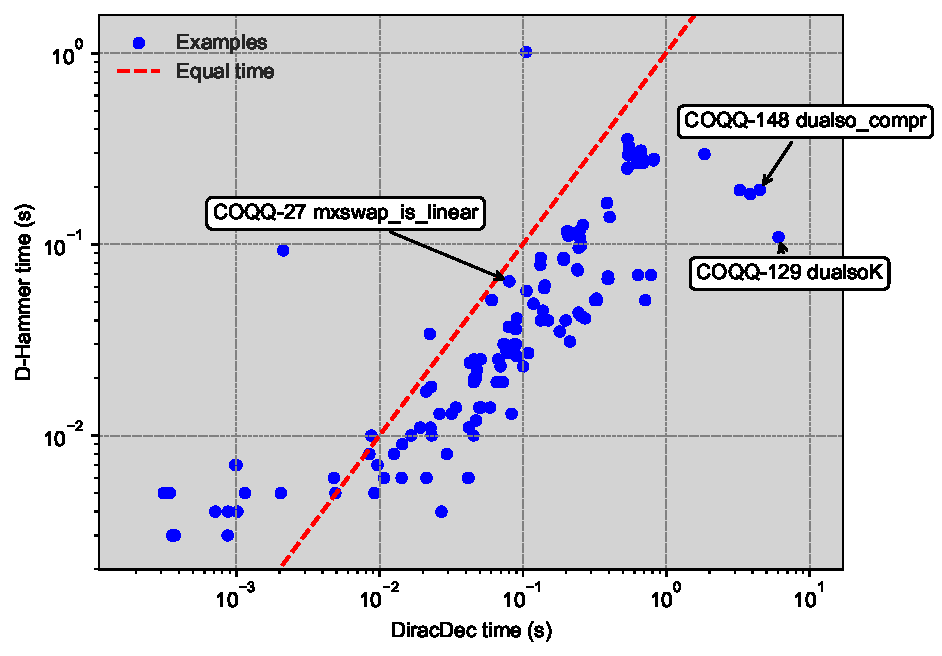
\includegraphics[width=0.8\textwidth]{fig/coqq.pdf}
    \caption{Time comparison between DiracDec and D-Hammer on the CoqQ benchmark.}
    \label{fig: CoqQ plot}
\end{figure}

\subsubsection{CoqQ}
As to expressibility, D-Hammer encodes 158 examples for the CoqQ part, 4 less than DiracDec. This is because the language for DiracDec has the support for projectors $\texttt{fst}$ and $\texttt{snd}$ on basis pairs, satisfying $\texttt{fst} (s, t) = s$ and $\texttt{snd} (s, t) = t$. We found this feature is almost not used and removed the support. For decidability, we improved the rewriting rules about sum for D-Hammer, and proved several more examples failed by DiracDec. 
\Cref{fig: CoqQ plot} shows a direct comparison of their time efficiency.
We can observe that for small examples, D-Hammer is slower because of the marginal overhead. 
When the running time goes up, D-Hammer provides 2 to 40 times of acceleration in average.
The relationship between efficiency improvement and example characteristics further supports the necessity of our algorithm. 
We find that examples with great efficiency improvement, e.g. COQQ-129 and COQQ-148 shown in~\Cref{fig: CoqQ plot}, tend to use deeply nested summations, where our algorithm has an effect.

% \subsubsection{Others}
% Other examples are taken from quantum circuits and one recent paper [TODO]. Because these examples involve decomposition on concrete $\ket{0}$ and $\ket{1}$ qubit basis, resulting a lot of addition elements, our algorithm dealing with AC symbols brings along significant improvement.
% One typical example is
% \begin{gather*}
%     (I \otimes P) \cdot U \cdot (I \otimes P) \cdot U^\dagger = \ket{0}\bra{0} \otimes I + \ket{1}\bra{1}\otimes (P \cdot P), \\
%     \textrm{where } P \triangleq e^{-i\theta/2} \ket{0}\bra{0} + e^{i\theta/2}\ket{1}\bra{1}, \qquad U \triangleq \ket{0}\bra{0} \otimes X + \ket{1}\bra{1} \otimes I.
% \end{gather*}
% It takes DiracDec about one minute, but D-Hammer solves it within one second.


\subsubsection{Labelled Dirac Notation}
We present a new set of examples for labelled Dirac notation (LDN), as detailed in~\Cref{sec: examples for labelled}. These examples, illustrated in~\Cref{fig: labelled examples}, include six representative cases drawn from a variety of sources, such as well-established theorems, research paper results, quantum circuit equivalence, and quantum program verification.
D-Hammer normalizes them and successfully checks their equivalence using the algorithm in~\Cref{sec: labelled}.
Among the examples, LDN-12 shows the flexibility in combining labelled Dirac notations.
Example LDN-14 and LDN-18 are about circuits or programs on qubits. LDN-14 shows how to calculate controlled-not gate in different ways. In LDN-18, $q, q_1$ and $q_2$ represent variables for quantum programs, and the equation shows the change of the state after applying $X$ gate on $q_2$. Experiments show that our algorithm is relatively inefficient for labelled Dirac notations based on qubits.

It is a noteworthy result that D-Hammer solved LDN-10, a highly complex and lengthy example. It is a theorem on quantum separation logic from~\cite{DBLP:conf/lics/ZhouBHYY21}, and is challenging to prove even for experts. Notice that 7 registers are involved here, and it would be impractical to organize and referring to the subsystems without using labels.

\begin{figure}[h]
    \center
    % \scriptsize
    \setlength{\extrarowheight}{2pt}
    \begin{tabular}{l c c l}
        \hline
        example & source & time(s) & equation \\
        \hline
        LDN-4 & theorem & 0.03 & \( \bra{\Phi}_{(x, y)} M_y \cdot N_x \ket{\Phi}_{(x, y)} = \mathrm{tr}(M^T N) \) \\
        LDN-10 & paper~\cite{DBLP:conf/lics/ZhouBHYY21} & 5.17 & \( \mathrm{tr}_{((a',(b,b')),c')}\Big[\mathrm{tr}_{r}\Big(U_{(r,(a,b))} \cdot\Big(|s\>_r\<s|\otimes 
        \Big[V_{((a',(b,b')),c')} \cdots \)\\
        LDN-11 & paper~\cite{PALSBERG2024206} & 0.12 & \( U_{(a,b)}\cdot W_{(b,c)}\cdot V_{(a,c)} = 
        \sum_i |i\>_a\<i|\otimes \big((P_i)_c\cdot W_{(b,c)}\cdot (Q_i)_c\big)\) \\
        LDN-12 & circuit & 0.07 & \( \ket{i}_{a;b}\bra{j} \cdot C_{(b,c)} \cdot D_{(c,d)} = {}_b\bra{j} \cdot C_{(b,c)} \cdot D_{(c,d)} \cdot \ket{i}_{a}\) \\
        LDN-14 & circuit & 7.37 & \scriptsize{\( \textsf{CNOT}_{rq}\ket{\textrm{GHZ}}_{pqr} = (\textsf{CNOT}\ket{00})_{rq}\ket{0}_p + (\textsf{CNOT}\ket{11})_{rq}\ket{1}_p \)} \\
        LDN-18 & program & 1.01 & \( -\ket{0}_q\ket{+-}_{q_1, q_2} = X_{q_2} \ket{0}_q\ket{+-}_{q_1, q_2} \) \\
        \hline
    \end{tabular}
    \caption{Part of examples for labelled Dirac notations.}
    \label{fig: labelled examples}
\end{figure}

\section{Related Work}

\paragraph*{Comparison with DiracDec~\cite{diracdec}}
Xu \emph{et al}~\cite{diracdec} define a language and an associate and
commutative rewriting system for Dirac notation, and implement their
language and rewriting system in Mathematica. Our approach follows a
similar pattern. However, there are significant differences in terms
of scope, expressiveness, and efficiency. We review these differences
below.

The most obvious difference is that D-Hammer targets labelled Dirac
notation, whereas DiracDec targets plain Dirac notation. As already
mentioned, the use of labelled Dirac notation is essential in many
applications; in particular, labelled Dirac notation can simplify
notation and proofs, and is in general better suited for writing and
reasoning about complex, many-body, quantum states. However, there are
several other important differences. First, our language leverages
higher-order functions to provide a compact and expressive
representation of big operators. Second, our language adopts AC
symbols with indefinite arities, which leads to compact representation
of terms, and eases AC reasoning. Third, the relation with Mathematica
is fundamentally different. DiracDec is implemented in Mathematica; as
a consequence, its behavior, and in particular, its typing rules are
constrained by the lack of typing in Mathematica. In contrast,
D-Hammer is designed as a separate tool; as a consequence, it benefits
from an improved representation of terms (e.g.\, AC operators with
indefinite arity), a more expressive type system (e.g.\, dependent
types), and a more efficient rewriting engine. D-Hammer still relies
on Mathematica to reason about functions that are not natively
supported by rewriting rules, but these interactions are constrained
and do not have negative effects on the overall efficiency of the
system. This is reflected in our experimental comparison of D-Hammer
and DiracDec, which shows how the former outperforms the latter.


\paragraph*{Comparison with ZX Calculus}
The ZX calculus~\cite{DBLP:conf/icalp/CoeckeD08,coecke2011interacting}
is a graphical calculus for quantum states. A main appeal of the ZX
calculus is that its foundations are grounded in categorical quantum
mechanics~\cite{DBLP:conf/lics/AbramskyC04}, a powerful framework for
modeling and reasoning about quantum physics. Another main appeal of
the ZX calculus is that ZX diagrams have an operational interpretation
using graph rewriting. There is a large body of work that studies
properties of these rewriting systems, and in particular completeness
(a set of rules is complete if it can prove all valid identities) and
minimality (a complete set of rules is minimal if removing a rule
leads to incompleteness). Two main proof techniques for completeness
are via termination, or via interpretation. In the first case, one
shows that a rewriting system has unique normal forms and that two
expressions are semantically equivalent iff they have the same normal
form---there exists many relaxations of this result---whereas in the
second case one shows completeness by exhibiting a well-behaved
translation to another system for which completeness holds. Both proof
techniques have been used to prove completeness for multiple settings,
including the Clifford fragment~\cite{backens2014zx}, the
Toffoli+Hadamard fragment~\cite{hadzi15zx}, the Clifford+T
fragment~\cite{jeandel2018complete} and the (qubit) universal
fragment~\cite{HNW18,JeandelPV18beyond}. Subsequent works generalize
completeness to qudits~\cite{Poor2023} for a calculus know as ZXW
which encompasses the ZX and ZW calculi~\cite{zwcalculus}. We refer
the reader to~\cite{vandewetering2020zx} for a (relatively) recent
historical and technical account of completeness results.

Because they are both grounded in rewriting techniques, there are many
similarities between prior work on the ZX calculus and our own work on
labelled Dirac notation. We highlight some key differences. First,
there exist a number of differences between our language and the
concrete fragments of the ZX-calculus for which completeness has been
studied. For instance, our language features big operators, and
operators for dual spaces. A second difference is that we do not claim
completeness: our main theorem shows a reduction from Labelled Dirac
notation to Dirac notation, for which completeness is only partially
known.




it is difficult to compare the ZX
calculus and LDN. First, they have different scopes: the ZX calculus
mainly focuses on quantum circuits, whereas LDN aims to provide
general support for quantum physics. This difference in scope is
reflected in the underlying languages: for instance, many works in ZX
calculus consider concrete sets of quantum gates, whereas LDN
emphasizes the use of big operators, and does not attempt to provide
specialized support for a particular set of quantum gates. As a
result, many of the examples handled by D-Hammer cannot be formalized
in existing ZX-calculus tools. On the contrary, D-Hammer is not
competitive on the examples that can be verified by ZX-calculus.

\gb{give a few examples in terms of size and time}

\paragraph*{Comparison with path-over sums approach}
Similarly, there exist
completeness results and tools for the sum-over-paths representation
of quantum states~\cite{amy2018towards,amy2023complete}.


\paragraph*{Comparison with equivalence checking}

Automata-based approaches has also been successfully applied for
reasoning about quantum circuits~\cite{AutoQ_pldi_2023}. Instead of
representing a set of $n$-qubit states in exponential size,
\cite{AutoQ_pldi_2023} encode it as (finite) tree automata with much
less (often $\mathit{poly}(n)$) transitions.  They further established
transformers to implement the semantics of quantum gates over this
representation, providing better scalability compared to other
approaches. It is developed as a practical tool \textsc{autoq} with
the capabilities for symbolic reasoning~\cite{AutoQ2023}. More
recently, \cite{AutoQ_popl2025} further explore level-synchronized
tree automata to encoding state, a promising model for parameterized
verification.


\paragraph*{Canonical forms in multi-body quantum physics}

\paragraph*{Comparison with egraphs}
Our algorithm is based on term rewriting. However, it is a challenge
to device well-behaved and efficient term rewriting for (labelled)
Dirac notation. An alternative to term rewriting would be to use
equality saturation~\cite{DBLP:journals/pacmpl/WillseyNWFTP21}, a
powerful equational reasoning technique that does not require
existence of normal forms. Equality saturation may be particularly
useful when considering further extensions of labelled Dirac notation.

%% The first step is to formalize the language for Dirac notation. In DiracDec, the language has a concrete design, where the same syntax for different types corresponds to distinct symbols. Our goal is to transition from this concrete design to a more abstract one, which aligns more closely with the conventional Dirac notation we use and simplifies the term rewriting system.

%% %% Automated theorem proving has seen significant advancements in recent years, particularly through the development of satisfiability modulo theories (SMT) solvers,
%% %% % SMT solvers extend propositional satisfiability by integrating theories such as arithmetic, arrays, and bit-vectors, making them suitable for solving a wide range of verification problems in both hardware and software domains. 
%% %% including prominent tools like Z3. These solvers have become essential in various fields such as formal verification, synthesis, and model checking. 
%% %% Equational reasoning is another crucial area of research within automated theorem proving, which focuses on solving problems that involve equations between terms in an algebraic structure. 
%% %% Equational provers, such as Vampire and E, have played a pivotal role in addressing the challenge of proving equations in first-order logic, employing sophisticated algorithms like superposition and term rewriting.

%% %% Formal verification of quantum computation is receiving increasing attentions during these years. See~\cite{Lewis2023} for a comprehensive review. 
%% %% Verification frameworks in Coq include the foundational formalization CoqQ and quantum circuit language QWIRE. 
%% %% Verifications of quantum programs are also considered, such as the Hoare logic based methods [] and model checking based methods [].
%% %% The equational reasoning of Dirac notation is crucial for establishing property proofs in these works.
%% %% Verification theoreis and tools based on other languages are also proposed, such as PyZX for reasoning and simplification of ZX-calculus.




\section{Conclusion and Future Work}
We have designed and implemented D-Hammer, a dependently typed
higher-order language and proof system for labelled Dirac
notation. D-Hammer benefits from an optimized implementation in
\CC\ and a tight integration with Mathematica to reason about a broad
range of mathematical functions, including trigonometric and
exponential functions, that are commonly used in quantum physics.
There are two important directions for future work. 
% The first
% direction is to enhance D-Hammer with support for big tensor notation,
% i.e.\, to support expressions of the form $\bigotimes_{i\in I}
% e_i$. 
The first direction is to extend D-Hammer with a mechanism to
generate independently verifiable certificates.  There is a large body
of work on producing certificates for automated tools, in particular
SMT solvers; see e.g.~\cite{DBLP:journals/cacm/BarbosaBCDKLNNOPRTZ23}
for a recent overview. One potential option would be to integrate
D-Hammer with the Coq or Lean proof assistants; in the first case, one
would benefit from the formalization of labelled Dirac notation in
CoqQ~\cite{Zhou2023}, whereas in the second case, one would benefit
from powerful mechanisms to integrate rewriting procedures into the
Lean proof assistant. The second direction is to connect
D-Hammer with quantum program verifiers. Two potential applications
are automating equational proofs for tools that already use Dirac
notation, and to substitute numerical methods for tools that use
matrices instead of symbolic assertions.




%% Based on the first equational reasoning tool for Dirac notation called DiracDec, this work improves and extends the theory for practical applications, and provides the solver D-Hammer. Experiments show that the tool demonstrates advantages in decidability, efficiency and usability. 

%% We expect D-Hammer to have applications in areas like quantum program verification or proofs of post-quantum cryptography protocols in the future.
%% One promising following up is to connect D-Hammer with theorem provers like Coq. It involves transforming theorem prover expressions into D-Hammer, and verify the proof trace of D-Hammer in theorem provers. Besids, most quantum program verifiers nowadays depend on matrix calculations. D-Hammer can serve as the replacement for matrix methods to enable symbolic deductions.





%%%%%%%%%%%%%%%%%%%%%%%%%%

% \begin{credits}
%     \subsubsection{\ackname} A bold run-in heading in small font size at the end of the paper is
%     used for general acknowledgments, for example: This study was funded
%     by X (grant number Y).
% \end{credits}
    
    


%
% ---- Bibliography ----
%
% BibTeX users should specify bibliography style 'splncs04'.
% References will then be sorted and formatted in the correct style.
%
\bibliographystyle{splncs04}
\bibliography{ref}
%

\appendix

\section{Full Typing Rules}

\label{sec: full typing rules}

This section includes the full list of typing rules.

\begin{itemize}
    \item Rules for a well-formed environment and context.
    \[
        \textbf{W-Empty} \qquad
        \frac{}{\WF([])[]}
    \]
    \[
        \textbf{W-AssumE-Index} \qquad
        \frac{\WF(E)[] \qquad x \notin E}{\WF(E; x : \Index)[]}
    \]
    \[
        \textbf{W-AssumE-Term} \qquad
        \frac{E[] \vdash T : \Type \qquad x \notin E}{\WF(E; x:T)[]}
    \]
    \[
        \textbf{W-Def-Term} \qquad
        \frac{E[]\vdash t:T \qquad x \notin E}{\WF(E; x:=t:T)[]}
    \]
    \[
        \textbf{W-AssumC-Index} \qquad
        \frac{\WF(E)[\Gamma]}{\WF(E)[\Gamma; x : \Index]}
    \]
    \[
        \textbf{W-AssumC-Term} \qquad
        \frac{E[\Gamma] \vdash T : \Type}{\WF(E)[\Gamma; x : T]}
    \]


    \item Rules for type indices.
    \[
        \textbf{Index-Var} \qquad
        \frac{\WF(E)[\Gamma] \qquad x : \Index \in E[\Gamma]}{E[\Gamma] \vdash x : \Index}
    \]
    \[
        \textbf{Index-Prod} \qquad
        \frac{E[\Gamma] \vdash \sigma : \Index \qquad E[\Gamma] \vdash \tau : \Index}{E[\Gamma] \vdash \sigma \times \tau : \Index}
    \]
    \[
        \textbf{Index-Qudit} \qquad
        \frac{\WF(E)[\Gamma]}{E[\Gamma] \vdash \mathsf{bool} : \Index}
    \]


    \item Rules for types.
    \[
        \textbf{Type-Lam} \qquad
        \frac{E[\Gamma] \vdash T : \Type \qquad E[\Gamma] \vdash U : \Type}{E[\Gamma] \vdash T \to U : \Type}
    \]
    \[
        \textbf{Type-Index} \qquad
        \frac{E[\Gamma ; x : \Index] \vdash U : \Type}{E[\Gamma] \vdash \forall x.U : \Type}
    \]
    \[
        \textbf{Type-Basis} \qquad
        \frac{E[\Gamma] \vdash \sigma : \Index}{E[\Gamma] \vdash \Basis(\sigma) : \Type}
    \]
    \[
        \textbf{Type-Ket} \qquad
        \frac{E[\Gamma] \vdash \sigma : \Index}{E[\Gamma] \vdash \KType(\sigma) : \Type}
    \]
    \[
        \textbf{Type-Bra} \qquad
        \frac{E[\Gamma] \vdash \sigma : \Index}{E[\Gamma] \vdash \BType(\sigma) : \Type}
    \]
    \[
        \textbf{Type-Opt} \qquad
        \frac{E[\Gamma] \vdash \sigma : \Index \qquad E[\Gamma] \vdash \tau : \Index}{E[\Gamma] \vdash \OType(\sigma, \tau) : \Type}
    \]
    \[
        \textbf{Type-Scalar} \qquad
        \frac{\WF(E)[\Gamma]}{E[\Gamma] \vdash \SType : \Type}
    \]
    \[
        \textbf{Type-Set} \qquad
        \frac{E[\Gamma] \vdash \sigma : \Index}{E[\Gamma] \vdash \SET(\sigma) : \Type}
    \]
    \[
        \textbf{Type-Register} \qquad
        \frac{E[\Gamma] \vdash  \sigma : \Index}{E[\Gamma] \vdash \reg(\sigma) : \Type}
    \]
    \[
        \textbf{Type-Labelled} \qquad
        \frac{E[\Gamma] \vdash r : \reg(\sigma_r) \text{ for all $r$ in $s_1$ and $s_2$} }{E[\Gamma] \vdash \DType(s_1, s_2) : \textsf{Type}} 
    \]

    \item Rules for variable and function typings. Here $U\{x/u\}$ means replacing the bound variable $x$ with $u$ in $U$.
    \[
        \textbf{Term-Var} \qquad
        \frac{
            \begin{aligned}
                & \WF(E)[\Gamma] \\
                & (x:T) \in E[\Gamma] \text{ or } (x := t : T) \in E \text{ for some $t$}
            \end{aligned}
        }
        {E[\Gamma] \vdash x : T}
    \]
    \[
        \textbf{Lam} \qquad
        \frac{E[\Gamma; x : T] \vdash t : U}{E[\Gamma] \vdash (\lambda x : T . t) : T \to U}
    \]
    \[
        \textbf{Index} \qquad
        \frac{E[\Gamma; x : \Index] \vdash t : U}{E[\Gamma] \vdash (\mu x.t) : \forall x.U}
    \]
    \[
        \textbf{App-Lam} \qquad
        \frac{E[\Gamma] \vdash t:U \to T \qquad E[\Gamma] \vdash u:U}{E[\Gamma] \vdash (t\ u):T}
    \]
    \[
        \textbf{App-Index} \qquad
        \frac{E[\Gamma] \vdash t:\forall x.U \qquad E[\Gamma] \vdash u : \Index}{E[\Gamma] \vdash (t\ u):U\{x/u\}}
    \]
    
    \item Basis term typing rules. 
    \[  \textbf{Basis-0} \qquad
        \frac{\WF(E[\Gamma])}{E[\Gamma] \vdash 0 : \Basis(\mathsf{bool})}
    \]
    \[  \textbf{Basis-1} \qquad
        \frac{\WF(E[\Gamma])}{E[\Gamma] \vdash 1 : \Basis(\mathsf{bool})}
    \]
    \[
        \textbf{Basis-Pair} \qquad
        \frac{E[\Gamma]\vdash s : \Basis(\sigma) \qquad E[\Gamma]\vdash t : \Basis(\tau)} {E[\Gamma]\vdash (s, t) : \Basis(\sigma \times \tau)}
    \]


    \item Composition typing rules. 
    \[  \textbf{Compo-SS} \qquad
        \frac{E[\Gamma] \vdash x : \SType \qquad E[\Gamma] \vdash y : \SType}{E[\Gamma] \vdash x \circ y : \SType}
    \]
    \[  \textbf{Compo-SK} \qquad
        \frac{E[\Gamma] \vdash x : \SType \qquad E[\Gamma] \vdash y : \KType(\sigma)}{E[\Gamma] \vdash x \circ y : \KType(\sigma)}
    \]
    \[  \textbf{Compo-SB} \qquad
        \frac{E[\Gamma] \vdash x : \SType \qquad E[\Gamma] \vdash y : \BType(\sigma)}{E[\Gamma] \vdash x \circ y : \BType(\sigma)}
    \]
    \[  \textbf{Compo-SO} \qquad
        \frac{E[\Gamma] \vdash x : \SType \qquad E[\Gamma] \vdash y : \OType(\sigma, \tau)}{E[\Gamma] \vdash x \circ y : \OType(\sigma, \tau)}
    \]
    \[  \textbf{Compo-KS} \qquad
        \frac{E[\Gamma] \vdash x : \KType(\sigma) \qquad E[\Gamma] \vdash y : \SType}{E[\Gamma] \vdash x \circ y : \KType(\sigma)}
    \]
    \[  \textbf{Compo-KK} \qquad
        \frac{E[\Gamma] \vdash x : \KType(\sigma) \qquad E[\Gamma] \vdash y : \KType(\tau)}{E[\Gamma] \vdash x \circ y : \KType(\sigma \times \tau)}
    \]
    \[  \textbf{Compo-KB} \qquad
        \frac{E[\Gamma] \vdash x : \KType(\sigma) \qquad E[\Gamma] \vdash y : \BType(\tau)}{E[\Gamma] \vdash x \circ y : \OType(\sigma, \tau)}
    \]
    \[  \textbf{Compo-BS} \qquad
        \frac{E[\Gamma] \vdash x : \BType(\sigma) \qquad E[\Gamma] \vdash y : \SType}{E[\Gamma] \vdash x \circ y : \BType(\sigma)}
    \]
    \[  \textbf{Compo-BK} \qquad
        \frac{E[\Gamma] \vdash x : \BType(\sigma) \qquad E[\Gamma] \vdash y : \KType(\sigma)}{E[\Gamma] \vdash x \circ y : \SType}
    \]
    \[  \textbf{Compo-BB} \qquad
        \frac{E[\Gamma] \vdash x : \BType(\sigma) \qquad E[\Gamma] \vdash y : \BType(\tau)}{E[\Gamma] \vdash x \circ y : \BType(\sigma \times \tau)}
    \]
    \[  \textbf{Compo-BO} \qquad
        \frac{E[\Gamma] \vdash x : \BType(\sigma) \qquad E[\Gamma] \vdash y : \OType(\sigma, \tau)}{E[\Gamma] \vdash x \circ y : \BType(\tau)}
    \]
    \[  \textbf{Compo-OS} \qquad
        \frac{E[\Gamma] \vdash x : \OType(\sigma, \tau) \qquad E[\Gamma] \vdash y : \SType}{E[\Gamma] \vdash x \circ y : \OType(\sigma, \tau)}
    \]
    \[  \textbf{Compo-OK} \qquad
        \frac{E[\Gamma] \vdash x : \OType(\sigma, \tau) \qquad E[\Gamma] \vdash y : \KType(\tau)}{E[\Gamma] \vdash x \circ y : \KType(\sigma)}
    \]
    \[  \textbf{Compo-OO} \qquad
        \frac{E[\Gamma] \vdash x : \OType(\sigma, \tau) \qquad E[\Gamma] \vdash y : \OType(\sigma', \tau')}{E[\Gamma] \vdash x \circ y : \OType(\sigma \times \sigma', \tau \times \tau')}
    \]
    \[
        \textbf{Compo-DD} \qquad
        \frac{
            \begin{aligned}
                E[\Gamma] \vdash x : \DType(s_1,s_1') \\
                E[\Gamma] \vdash y : \DType(s_2,s_2')
            \end{aligned}
            \qquad 
            \begin{aligned}
                s_1 \cap s_2 \backslash s_1' = \emptyset \\
                s_2' \cap s_1' \backslash s_2 = \emptyset
            \end{aligned}
        }
        {E[\Gamma] \vdash x\circ y : \DType(s_1 \cup (s_2\backslash s_1'), s_2' \cup (s_1'\backslash s_2))}
    \]


    \item Scalar term typing rules.
    \[
        \textbf{Sca-0} \qquad
        \frac{\WF(E)[\Gamma]}{E[\Gamma] \vdash 0 : \SType}
    \]
    \[
        \textbf{Sca-1} \qquad
        \frac{\WF(E)[\Gamma]}{E[\Gamma] \vdash 1 : \SType}
    \]
    \[
        \textbf{Sca-Delta} \qquad
        \frac{ E[\Gamma]\vdash s : \Basis(\sigma) \qquad E[\Gamma]\vdash t : \Basis(\sigma) } {E[\Gamma] \vdash \delta_{s, t} : \SType}
    \]
    \[
        \textbf{Sca-Add} \qquad
        \frac{E[\Gamma]\vdash a_i : \SType \text{ for all $i$}}{E[\Gamma]\vdash a_1 + \cdots + a_n : \SType}
    \]
    \[
        \textbf{Sca-Mul} \qquad
        \frac{E[\Gamma]\vdash a_i : \SType \text{ for all $i$}}{E[\Gamma]\vdash a_1 \times \cdots \times a_n : \SType}
    \]
    \[
        \textbf{Sca-Conj} \qquad
        \frac{E[\Gamma] \vdash a : \SType}{E[\Gamma] \vdash a^*:\SType}
    \]
    \[
        \textbf{Sca-Dot} \qquad
        \frac{E[\Gamma]\vdash B : \BType(\sigma) \qquad E[\Gamma]\vdash K : \KType(\sigma)}{E[\Gamma] \vdash B \cdot K : \SType}
    \]
    \[
        \textbf{Sca-Sum} \qquad
        \frac{E[\Gamma] \vdash s : \SET(\sigma) \qquad E[\Gamma] \vdash f : \Basis(\sigma) \to \SType}{E[\Gamma] \vdash \sum_{s} f : \SType}
    \]

    \item Ket term typing rules.
    \[
        \textbf{Ket-0} \qquad
        \frac{E[\Gamma] \vdash \sigma : \Index}{E[\Gamma] \vdash \ZEROK(\sigma) : \KType(\sigma)}
    \]
    \[
        \textbf{Ket-Basis} \qquad
        \frac{E[\Gamma]\vdash t : \Basis(\sigma)}{E[\Gamma] \vdash \ket{t} : \KType(\sigma)}
    \]
    \[
        \textbf{Ket-Adj} \qquad
        \frac{E[\Gamma] \vdash B : \BType(\sigma)}{E[\Gamma] \vdash B^\dagger : \KType(\sigma)}
    \]
    \[
        \textbf{Ket-Scr} \qquad
        \frac{E[\Gamma] \vdash a : \SType \qquad E[\Gamma] \vdash K : \KType(\sigma)}{E[\Gamma] \vdash a.K : \KType(\sigma)}
    \]
    \[
        \textbf{Ket-Add} \qquad
        \frac{E[\Gamma] \vdash K_i : \KType(\sigma) \text{ for all $i$}}{E[\Gamma] \vdash K_1 + \cdots + K_n : \KType(\sigma)}
    \]
    \[
        \textbf{Ket-MulK} \qquad
        \frac{E[\Gamma] \vdash O : \OType(\sigma, \tau) \qquad E[\Gamma] \vdash K : \KType(\tau)}{E[\Gamma] \vdash O \cdot K : \KType(\sigma)}
    \]
    \[
        \textbf{Ket-Tsr} \qquad
        \frac{E[\Gamma] \vdash K_1 : \KType(\sigma) \qquad E[\Gamma] \vdash K_2 : \KType(\tau)} {E[\Gamma] \vdash K_1 \otimes K_2 : \KType(\sigma \times \tau)}
    \]
    \[
        \textbf{Ket-Sum} \qquad
        \frac{E[\Gamma] \vdash s : \SET(\sigma) \qquad E[\Gamma] \vdash f : \Basis(\sigma) \to \KType(\tau)}{E[\Gamma] \vdash \sum_{s} f : \KType(\tau)}
    \]

    \item Bra term typing rules.
    \[
        \textbf{Bra-0} \qquad
        \frac{E[\Gamma] \vdash \sigma : \Index}{E[\Gamma] \vdash \ZEROB(\sigma) : \BType(\sigma)}
    \]
    \[
        \textbf{Bra-Basis} \qquad
        \frac{E[\Gamma]\vdash t : \Basis(\sigma)}{E[\Gamma] \vdash \bra{t} : \BType(\sigma)}
    \]
    \[
        \textbf{Bra-Adj} \qquad
        \frac{E[\Gamma] \vdash K : \KType(\sigma)}{E[\Gamma] \vdash K^\dagger : \BType(\sigma)}
    \]
    \[
        \textbf{Bra-Scr} \qquad
        \frac{E[\Gamma] \vdash a : \SType \qquad E[\Gamma] \vdash B : \BType(\sigma)}{E[\Gamma] \vdash a.B : \BType(\sigma)}
    \]
    \[
        \textbf{Bra-Add} \qquad
        \frac{E[\Gamma] \vdash B_i : \BType(\sigma) \text{ for all $i$}}{E[\Gamma] \vdash B_1 + \cdots + B_n : \BType(\sigma)}
    \]
    \[
        \textbf{Bra-MulB} \qquad
        \frac{E[\Gamma] \vdash B : \KType(\sigma) \qquad E[\Gamma] \vdash O : \OType(\sigma, \tau)}{E[\Gamma] \vdash B \cdot O : \BType(\tau)}
    \]
    \[
        \textbf{Bra-Tsr} \qquad
        \frac{E[\Gamma] \vdash B_1 : \BType(\sigma) \qquad E[\Gamma] \vdash B_2 : \BType(\tau)} {E[\Gamma] \vdash B_1 \otimes B_2 : \BType(\sigma \times \tau)}
    \]
    \[
        \textbf{Bra-Sum} \qquad
        \frac{E[\Gamma] \vdash s : \SET(\sigma) \qquad E[\Gamma] \vdash f : \Basis(\sigma) \to \BType(\tau)}{E[\Gamma] \vdash \sum_{s} f : \BType(\tau)}
    \]

    \item Operator term typing rules.
    \[
        \textbf{Opt-0} \qquad
        \frac{E[\Gamma] \vdash \sigma : \Index \qquad E[\Gamma] \vdash \tau : \Index}{E[\Gamma] \vdash \ZEROO(\sigma, \tau) : \OType(\sigma, \tau)}
    \]
    \[
        \textbf{Opt-1} \qquad
        \frac{E[\Gamma] \vdash \sigma : \Index}{E[\Gamma] \vdash \ONEO(\sigma) : \OType(\sigma, \sigma)}
    \]
    \[
        \textbf{Opt-Adj} \qquad
        \frac{E[\Gamma] \vdash O : \OType(\sigma, \tau)}{E[\Gamma] \vdash O^\dagger : \OType(\tau, \sigma)}
    \]
    \[
        \textbf{Opt-Scr} \qquad
        \frac{E[\Gamma] \vdash a : \SType \qquad E[\Gamma] \vdash O : \OType(\sigma, \tau)}{E[\Gamma] \vdash a.O : \OType(\sigma, \tau)}
    \]
    \[
        \textbf{Opt-Add} \qquad
        \frac{E[\Gamma] \vdash O_i : \OType(\sigma, \tau) \text{ for all $i$}}{E[\Gamma] \vdash O_1 + \cdots + O_n : \OType(\sigma, \tau)}
    \]
    \[
        \textbf{Opt-Outer} \qquad
        \frac{E[\Gamma]\vdash K : \KType(\sigma) \qquad E[\Gamma]\vdash B : \BType(\tau)}{E[\Gamma]\vdash K \cdot B : \OType(\sigma, \tau)}
    \]
    \[
        \textbf{Opt-Mulo} \qquad
        \frac{E[\Gamma] \vdash O_1 : \OType(\sigma, \tau) \qquad E[\Gamma] \vdash O_2 : \OType(\tau, \rho)}{E[\Gamma] \vdash O_1 \cdot O_2 : \OType(\sigma, \rho)}
    \]
    \[
        \textbf{Opt-Tsr} \qquad
        \frac{E[\Gamma] \vdash O_1 : \OType(\sigma_1, \tau_1) \qquad E[\Gamma] \vdash O_2 : \OType(\sigma_2, \tau_2)} {E[\Gamma] \vdash O_1 \otimes O_2 : \OType(\sigma_1 \times \sigma_2, \tau_1 \times \tau_2)}
    \]
    \[
        \textbf{Opt-Sum} \qquad
        \frac{E[\Gamma] \vdash s : \SET(\sigma) \qquad E[\Gamma] \vdash f : \Basis(\sigma) \to \OType(\tau, \rho)}{E[\Gamma] \vdash \sum_{s} f : \OType(\tau, \rho)}
    \]

    \item Set term typing rules.
    \[
        \textbf{Set-U} \qquad
        \frac{E[\Gamma] \vdash \sigma : \Index}{E[\Gamma] \vdash \mathbf{U}(\sigma) : \SET(\sigma)}
    \]
    \[
        \textbf{Set-Prod} \qquad
        \frac{E[\Gamma] \vdash A : \SET(\sigma) \qquad E[\Gamma] \vdash B : \SET(\tau)}{E[\Gamma] \vdash A \star B : \SET(\sigma \times \tau)}
    \]


    \item Register term typing rules.
    \[
        \textbf{Reg-Var} \qquad
        \frac{\WF(E[\Gamma]) \qquad r : \reg(\sigma) \in E}{E[\Gamma] \vdash r : \reg(\sigma)}
    \]
    \[
        \textbf{Reg-Pair}\qquad
        \frac{
            \begin{aligned}
                E[\Gamma] \vdash R : \reg(\sigma) \\
                E[\Gamma] \vdash Q : \reg(\tau)
            \end{aligned}
            \qquad \var(R) \cap \var(Q) = \emptyset
        }{E[\Gamma] \vdash (R,Q) : \reg(\sigma \times \tau)}
    \]

    \item Typing rules for labelled Dirac notations.
    \[
        \textbf{L-Basis-Ket}\qquad 
        \frac{r : \reg(\sigma) \in E\qquad E[\Gamma] \vdash i : \Basis(\sigma)}{E[\Gamma] \vdash |i\>_r : \DType(\{r\}, \emptyset)}
    \]
    \[
        \textbf{L-Basis-Bra}\qquad 
        \frac{r : \reg(\sigma) \in E \qquad E[\Gamma] \vdash i : \Basis(\sigma)}{E[\Gamma] \vdash {}_r\<i| : \DType(\emptyset, \{r\})}
    \]
    \[
        \textbf{L-Ket}\qquad 
        \frac{E[\Gamma] \vdash R : \reg(\sigma)\qquad E[\Gamma] \vdash K : \KType(\sigma)}{E[\Gamma] \vdash K_R : \DType(\var R, \emptyset)}
    \]
    \[
        \textbf{L-Bra}\qquad 
        \frac{E[\Gamma] \vdash R : \reg(\sigma)\qquad E[\Gamma] \vdash B : \BType(\sigma)}{E[\Gamma] \vdash B_R : \DType(\emptyset, \var R)}
    \]
    \[
        \textbf{L-Opt}\qquad 
        \frac{
            \begin{aligned}
                E[\Gamma] \vdash R_1 : \reg (\sigma_1) \\
                E[\Gamma] \vdash R_2 : \reg (\sigma_2)
            \end{aligned}
            \qquad
            E[\Gamma] \vdash O : \OType(\sigma_1, \sigma_2)
        }
        {E[\Gamma] \vdash O_{R_1;R_2} : \DType(\var R_1, \var R_2)}
    \]
    \[
        \textbf{L-Conj}\qquad 
        \frac{E[\Gamma] \vdash D : \DType(s_1,s_2)}{E[\Gamma] \vdash D^\dagger : \DType(s_2,s_1)}
    \]
    \[
        \textbf{L-Scl}\qquad 
        \frac{E[\Gamma] \vdash S : \SType\qquad E[\Gamma] \vdash D : \DType(s_1,s_2)}{E[\Gamma] \vdash S.D : \DType(s_1,s_2)}
    \]
    \[
        \textbf{L-Add}\qquad
        \frac{E[\Gamma] \vdash D_i : \DType(s_1,s_2)\quad \text{forall } i}{E[\Gamma] \vdash D_1+\cdots+D_n : \DType(s_1,s_2)}
    \]
    \[
        \textbf{L-Tsr}\qquad
        \frac{
            E[\Gamma] \vdash D_i : \DType(s_i,s_i') \qquad
            \bigcap_i s_i = \emptyset \qquad
            \bigcap_i s_i' = \emptyset
        }
        {E[\Gamma] \vdash D_1 \otimes \cdots \otimes D_i : \DType(\bigcup_i s_i, \bigcup_i s_i')}
    \]
    \[
        \textbf{L-Dot}\qquad
        \frac{
            \begin{aligned}
                E[\Gamma] \vdash D_1 : \DType(s_1,s_1') \\
                E[\Gamma] \vdash D_2 : \DType(s_2,s_2')
            \end{aligned}
            \qquad 
            \begin{aligned}
                s_1 \cap s_2 \backslash s_1' = \emptyset \\
                s_2' \cap s_1' \backslash s_2 = \emptyset
            \end{aligned}
        }
        {E[\Gamma] \vdash D_1\cdot D_2 : \DType(s_1 \cup (s_2\backslash s_1'), s_2' \cup (s_1'\backslash s_2))}
    \]
    \[
        \textbf{L-Sum}\qquad
        \frac{E[\Gamma] \vdash s : \SET(\sigma) \qquad E[\Gamma] \vdash f : \Basis(\sigma) \to \DType(s_1, s_2)}{E[\Gamma] \vdash \sum_{s} f : \DType(s_1, s_2)}
    \]

\end{itemize}


\section{Axiomatic Semantics}

The full list of equational axioms are provided below.
    \begin{align*}
        & \textsc{(Ax-Scalar)} &&
        (B \cdot K)^* = K^\dagger \cdot B^\dagger
        \\
            & \textsc{(Ax-Delta)} &&
        \delta_{s, t}^* = \delta_{s, t}
        \qquad
        \bra{s} \cdot \ket{t} = \delta_{s, t}
        \\ & &&
        \delta_{s, s} = 1
        \qquad
        s \neq t \vdash \delta_{s, t} = 0
        \qquad
        \delta_{s, t} = \delta_{t, s}
        \\
            & \textsc{(Ax-Linear)} &&
        \mathbf{0} + D = D
        \qquad
        D_1 + D_2 = D_2 + D_1
        \\ & &&
        (D_1 + D_2) + D_3 = D_1 + (D_2 + D_3)
        \\ & &&
        0.D = \mathbf{0}
        \qquad
        a.\mathbf{0} = \mathbf{0}
        \qquad
        1.D = D
        \\ & &&
        a.(b.D) = (a \times b).D
        \qquad
        (a + b).D = a.D + b.D
        \\ & &&
        a.(D_1 + D_2) = a.D_1 + a.D_2
        \\
        & \textsc{(Ax-Bilinear)} &&
        D \cdot \mathbf{0} = \mathbf{0} 
        \qquad
        D_1 \cdot (a.D_2) = a.(D_1 \cdot D_2)
        \\ & &&
        D_0 \cdot (D_1 + D_2) = D_0 \cdot D_1 + D_0 \cdot D_2
        \\ & &&
        \mathbf{0} \cdot D = \mathbf{0}
        \qquad
        (a.D_1) \cdot D_2 = a.(D_1 \cdot D_2)
        \\ & &&
        (D_1 + D_2) \cdot D_0 = D_1 \cdot D_0 + D_2 \cdot D_0
        \\ 
        & &&
        D \otimes \mathbf{0} = \mathbf{0}
        \qquad
        D_1 \otimes (a.D_2) = a.(D_1 \otimes D_2)
        \\ & &&
        D_0 \otimes (D_1 + D_2) = D_0 \otimes D_1 + D_0 \otimes D_2
        \\ & &&
        \mathbf{0} \otimes D = \mathbf{0} 
        \qquad
        (a.D_1) \otimes D_2 = a.(D_1 \otimes D_2)
        \\ & &&
        (D_1 + D_2) \otimes D_0 = D_1 \otimes D_0 + D_2 \otimes D_0
        \\ 
            & \textsc{(Ax-Adjoint)} &&
        \mathbf{0}^\dagger = \mathbf{0}
        \qquad
        (D^\dagger)^\dagger = D 
        \qquad
        (a.D)^\dagger = a^*.(D^\dagger)
        \\ & &&
        (D_1 + D_2)^\dagger = D_1^\dagger + D_2^\dagger
        \\
        & && (D_1 \cdot D_2)^\dagger = D_2^\dagger \cdot D_1^\dagger
        \qquad
        (D_1 \otimes D_2)^\dagger = D_1^\dagger \otimes D_2^\dagger
        \\
            & \textsc{(Ax-Comp)} &&
        D_0 \cdot (D_1 \cdot D_2) = (D_0 \cdot D_1) \cdot D_2
        \\ & &&
        (D_1 \otimes D_2) \cdot (D_3 \otimes D_4) = (D_1 \cdot D_3) \otimes (D_2 \cdot D_4)
        % \\ & &&
        % (K_1 \cdot B_1) \cdot (K_2 \cdot B_2) = (B_1 \cdot K_2) . (K_1 \otimes B_2)
        \\ & &&
        (K_1 \cdot B) \cdot K_2 = (B \cdot K_2).K_1
        \qquad
        B_1 \cdot (K \cdot B_2) = (B_1 \cdot K).B_2
        % \\ & &&
        % (K \cdot B) \cdot O = K \cdot (B \cdot O)
        % \qquad
        % O \cdot (K \cdot B) = (O \cdot  K) \cdot B
        % \\
        %     & &&
        % (K_1 \cdot B_1) \otimes (K_2 \cdot B_2) = (K_1 \otimes K_2) \cdot (B_1 \otimes B_2)
        \\ 
            & &&
        (B_1 \otimes B_2) \cdot (K_1 \otimes K_2) = (B_1 \cdot K_1) \times (B_2 \cdot K_2)
        \\ 
            & \textsc{(Ax-Ground)} &&
        \mathbf{1}_\mathcal{O}^\dagger = \mathbf{1}_\mathcal{O}
        \qquad
        \textbf{1}_\mathcal{O} \cdot D = D 
        \qquad
        \mathbf{1}_\mathcal{O} \otimes \mathbf{1}_\mathcal{O} = \mathbf{1}_\mathcal{O} 
        \\ & &&
        \ket{t}^\dagger = \bra{t}
        \qquad
        \ket{s} \otimes \ket{t} =\ket{(s, t)} 
    \end{align*}
\yx{to be continued}




\section{Rewriting Rules}

\label{sec: rewriting rules}

This section includes all the rewriting rules used in the system. Related rules are collected in the same table. 

\renewcommand{\arraystretch}{1.2} % Increases row height by 50%

\begin{ruletable}{Reductions for the definitions and function applications.}
    %
    BETA-ARROW
    & $((\lambda x : T.t)\ u)\ \reduce\ t\{x/u\}$ \\
    %
    BETA-INDEX
    & $((\mu x.t)\ u)\ \reduce\ t\{x/u\}$ \\
    %
    DELTA
    & $(c:=t:T) \in E \Rightarrow c\ \reduce\ t$
\end{ruletable}

\begin{ruletable}{The special to flatten all AC symbols within one call.}
    %
    R-FLATTEN
    & $a_1 + \cdots + (b_1 + \cdots + b_m) + \cdots + a_n$ \\
    & $\reduce\ a_1 + \cdots + b_1 + \cdots + b_m + \cdots + a_n$ \\ 
    \\
    & $a_1 \times \cdots \times (b_1 \times \cdots \times b_m) \times \cdots \times a_n$ \\
    & $\reduce\ a_1 \times \cdots \times b_1 \times \cdots \times b_m \times \cdots \times a_n$ \\
    \\
    & $X_1 + \cdots + (X_1' + \cdots + X_m') + \cdots + X_n$ \\
    & $\reduce\ X_1 + \cdots + X_1' + \cdots + X_m' + \cdots + X_n$
\end{ruletable}

\begin{ruletable}{Rules for scalar symbols.}
    %
    R-CONJ5
    & $ \delta_{s, t}^* \ \reduce\ \delta_{s, t}$ \\
    %
    R-CONJ6
    & $ (B \cdot K)^* \ \reduce\ K^\dagger \cdot B^\dagger $ \\
    %
    R-DOT0
    & $ \ZEROB(\sigma) \cdot K \ \reduce\ 0 $ \\
    %
    R-DOT1
    & $ B \cdot \ZEROK(\sigma) \ \reduce\ 0 $ \\
    %
    R-DOT2
    & $ (a.B) \cdot K \ \reduce\ a \times (B \cdot K) $ \\
    %
    R-DOT3
    & $ B \cdot (a.K) \ \reduce\ a \times (B \cdot K) $ \\
    %
    R-DOT4
    & $ (B_1 + \cdots + B_n) \cdot K \ \reduce\ B_1 \cdot K + \cdots + B_n \cdot K $ \\
    %
    R-DOT5
    & $ B \cdot (K_1 + \cdots + K_n) \ \reduce\ B \cdot K_1 + \cdots + B \cdot K_n $ \\
    %
    R-DOT6
    & $ \bra{s} \cdot \ket{t} \ \reduce\ \delta_{s, t} $ \\
    %
    R-DOT7
    & $ (B_1 \otimes B_2) \cdot \ket{(s, t)} \ \reduce\ (B_1 \cdot \ket{s}) \times (B_2 \cdot \ket{t}) $ \\
    %
    R-DOT8
    & $ \bra{(s, t)} \cdot (K_1 \otimes K_2) \ \reduce\ (\bra{s} \cdot K_1) \times (\bra{t} \cdot K_2) $ \\
    %
    R-DOT9
    & $ (B_1 \otimes B_2) \cdot (K_1 \otimes K_2) \ \reduce\ (B_1 \cdot K_1) \times (B_2 \cdot K_2) $ \\
    %
    R-DOT10
    & $ (B \cdot O) \cdot K \ \reduce\ B \cdot (O \cdot K) $ \\
    %
    R-DOT11
    & $ \bra{(s, t)} \cdot ((O_1 \otimes O_2) \cdot K) \ \reduce\ ((\bra{s} \cdot O_1) \otimes (\bra{t} \cdot O_2)) \cdot K $ \\
    %
    R-DOT12
    & $ (B_1 \otimes B_2) \cdot ((O_1 \otimes O_2) \cdot K) \ \reduce\ ((B_1 \cdot O_1) \otimes (B_2 \cdot O_2)) \cdot K $ \\
    %
    R-DELTA0
    & $ \delta_{a, a} \ \reduce\ 1$ \\
    %
    R-DELTA1
    & $ \delta_{(a, b), (c, d)} \ \reduce\ \delta_{a, c} \times \delta_{b, d}$ \\
\end{ruletable}


\begin{ruletable}{Rules for scaling.}
    %
    R-SCR0
    & $ 1.X \ \reduce\ X $ \\
    %
    R-SCR1
    & $ a.(b.X) \ \reduce\ (a \times b).X $ \\
    %
    R-SCR2
    & $ a.(X_1 + \cdots + X_n) \ \reduce\ a.X_1 + \cdots + a.X_n $ \\
    %
    R-SCRK0
    & $ K : \KType(\sigma) \Rightarrow 0.K \ \reduce\ \ZEROK(\sigma)$ \\
    %
    R-SCRK1
    & $ a.\ZEROK(\sigma) \ \reduce\ \ZEROK(\sigma) $ \\
    % 
    R-SCRB0
    & $ B : \BType(\sigma) \Rightarrow 0.B \ \reduce\ \ZEROB(\sigma)$ \\
    % 
    R-SCRB1
    & $ a.\ZEROB(\sigma) \ \reduce\ \ZEROB(\sigma) $ \\
    % 
    R-SCRO0
    & $ O : \OType(\sigma, \tau) \Rightarrow 0.O \ \reduce\ \ZEROO(\sigma, \tau)$ \\
    % 
    R-SCRO1
    & $ a.\ZEROO(\sigma, \tau) \ \reduce\ \ZEROO(\sigma, \tau) $ \\
\end{ruletable}

\begin{ruletable}{Rules for addition. }
    %
    R-ADDID
    & $+(X) \ \reduce\ X$ \\
    %
    R-ADD0
    & $Y_1 + \cdots + X + \cdots + X + \cdots + Y_n \ \reduce\ Y_1 + \cdots + Y_n + \cdots + (1+1).X$ \\
    %
    R-ADD1
    & $Y_1 + \cdots + X + \cdots + a.X + \cdots + Y_n \ \reduce\ Y_1 + \cdots + Y_n + (1+a).X$ \\
    %
    R-ADD2
    & $Y_1 + \cdots + a.X + \cdots + X + \cdots + Y_n \ \reduce\ Y_1 + \cdots + Y_n + (a+1).X$ \\
    %
    R-ADD3
    & $Y_1 + \cdots + a.X + \cdots + b.X + \cdots + Y_n \ \reduce\ Y_1 + \cdots + Y_n + (a+b).X$ \\
    %
    R-ADDK0
    & $K_1 + \cdots + \ZEROK(\sigma) + \cdots + K_n\ \reduce K_1 + \cdots + K_n$ \\
    %
    R-ADDB0
    & $B_1 + \cdots + \ZEROB(\sigma) + \cdots + B_n \ \reduce\ B_1 + \cdots + B_n$ \\
    %
    R-ADDO0
    & $O_1 + \cdots + \ZEROO(\sigma, \tau) + \cdots + O_n \ \reduce\ O_1 + \cdots + O_n$ 
    \\
\end{ruletable}

\begin{ruletable}{Rules for adjoint.}
    %
    R-ADJ0
    & $ (X^\dagger)^\dagger \ \reduce\ X $ \\
    %
    R-ADJ1
    & $ (a.X)^\dagger \ \reduce\ (a^*).(X^\dagger) $ \\
    %
    R-ADJ2
    & $ (X_1 + \cdots + X_n)^\dagger \ \reduce\ X_1^\dagger + \cdots + X_n^\dagger $ \\
    %
    R-ADJ3
    & $ (X \otimes Y)^\dagger \ \reduce\ X^\dagger \otimes Y^\dagger$ \\
    %
    R-ADJK0
    & $ \ZEROB(\sigma)^\dagger \ \reduce\ \ZEROK(\sigma) $ \\
    %
    R-ADJK1
    & $ \bra{t}^\dagger \ \reduce\ \ket{t} $ \\
    %
    R-ADJK2
    & $ (B \cdot O)^\dagger\ \reduce\ O^\dagger \cdot B^\dagger $ \\
    %
    R-ADJB0
    & $ \ZEROK(\sigma)^\dagger \ \reduce\ \ZEROB(\sigma) $ \\
    %
    R-ADJB1
    & $ \ket{t}^\dagger \ \reduce\ \bra{t} $ \\
    %
    R-ADJB2
    & $ (O \cdot K)^\dagger\ \reduce\ K^\dagger \cdot O^\dagger $ \\
    %
    R-ADJO0
    & $ \ZEROO(\sigma, \tau)^\dagger \ \reduce\ \ZEROO(\tau, \sigma) $ \\
    %
    R-ADJO1
    & $ \ONEO(\sigma)^\dagger \ \reduce\ \ONEO(\sigma)$ \\
    %
    R-ADJO2
    & $ (K \cdot B)^\dagger \ \reduce\ B^\dagger \cdot K^\dagger$ \\
    %
    R-ADJO3
    & $ (O_1 \cdot O_2)^\dagger \ \reduce\ O_2^\dagger \cdot O_1^\dagger $ \\
\end{ruletable}

\begin{ruletable}{Rules for tensor product.}
    R-TSR0
    & $ (a.X_1) \otimes X_2 \ \reduce\ a.(X_1 \otimes X_2) $ \\
    %
    R-TSR1
    & $ X_1 \otimes (a.X_2) \ \reduce\ a.(X_1 \otimes X_2) $ \\
    %
    R-TSR2
    & $ (X_1 + \cdots + X_n) \otimes X' \reduce X_1 \otimes X' + \cdots + X_n \otimes X' $ \\
    %
    R-TSR3
    & $ X' \otimes (X_1 + \cdots + X_n) \reduce X' \otimes X_1 + \cdots + X' \otimes X_n $ \\
    %
    R-TSRK0
    & $ K : \KType(\tau) \Rightarrow \ZEROK(\sigma) \otimes K\ \reduce\ \ZEROK(\sigma \times \tau) $ \\
    %
    R-TSRK1
    & $ K : \KType(\tau) \Rightarrow K \otimes \ZEROK(\sigma)\ \reduce\ \ZEROK(\tau \times \sigma) $ \\
    %
    R-TSRK2
    & $\ket{s} \otimes \ket{t} \ \reduce\ \ket{(s, t)}$ \\
    %
    R-TSRB0
    & $ B : \BType(\tau) \Rightarrow \ZEROB(\sigma) \otimes B\ \reduce\ \ZEROB(\sigma \times \tau) $ \\
    %
    R-TSRB1
    & $ B : \BType(\tau) \Rightarrow B \otimes \ZEROB(\sigma)\ \reduce\ \ZEROB(\tau \times \sigma) $ \\
    %
    R-TSRB2
    & $\bra{s} \otimes \bra{t} \ \reduce\ \bra{(s, t)}$ \\
    %
    R-TSRO0
    & $ O : \OType(\sigma, \tau) \Rightarrow O \otimes \ZEROO(\sigma', \tau') \ \reduce\ \ZEROO(\sigma \times \sigma', \tau \times \tau') $ \\
    % 
    R-TSRO1
    & $ O : \OType(\sigma, \tau) \Rightarrow \ZEROO(\sigma', \tau') \otimes O \ \reduce\ \ZEROO(\sigma' \times \sigma, \tau' \times \tau) $ \\
    %
    R-TSRO2
    & $\ONEO(\sigma) \otimes \ONEO(\tau)\ \reduce\ \ONEO(\sigma \times \tau)$ \\
    %
    R-TSRO3
    & $ (K_1 \cdot B_1) \otimes (K_2 \cdot B_2)\ \reduce\ (K_1 \otimes K_2) \cdot (B_1 \otimes B_2) $ \\
    %
\end{ruletable}

\begin{ruletable}{Rule for $O\cdot K$.}
    %
    R-MULK0
    & $ \ZEROO(\sigma, \tau) \cdot K \ \reduce\ \ZEROK(\sigma) $ \\
    %
    R-MULK1
    & $ O : \OType(\sigma, \tau) \Rightarrow O \cdot \ZEROK(\tau) \ \reduce\ \ZEROK(\sigma) $ \\
    %
    R-MULK2
    & $ \ONEO(\sigma) \cdot K \ \reduce K $ \\
    %
    R-MULK3
    & $ (a.O) \cdot K \ \reduce\ a.(O \cdot K) $ \\
    %
    R-MULK4
    & $ O \cdot (a.K) \ \reduce\ a.(O \cdot K) $ \\
    %
    R-MULK5
    & $ (O_1 + \cdots + O_n) \cdot K \ \reduce\ O_1 \cdot K + \cdots + O_n \cdot K $ \\
    %
    R-MULK6
    & $ O \cdot (K_1 + \cdots + K_n) \ \reduce\ O \cdot K_1 + \cdots + O \cdot K_n $ \\
    %
    R-MULK7
    & $ (K_1 \cdot B) \cdot K_2 \ \reduce\ (B \cdot K_2).K_1 $ \\
    %
    R-MULK8
    & $ (O_1 \cdot O_2) \cdot K \ \reduce\ O_1 \cdot (O_2 \cdot K) $ \\
    %
    R-MULK9
    & $ (O_1 \otimes O_2) \cdot ((O_1' \otimes O_2') \cdot K)\ \reduce\ ((O_1 \cdot O_1') \otimes (O_2 \cdot O_2')) \cdot K $ \\
    %
    R-MULK10
    & $ (O_1 \otimes O_2) \cdot \ket{(s, t)}\ \reduce\ (O_1 \cdot \ket{s}) \otimes (O_2 \cdot \ket{t}) $ \\
    %
    R-MULK11
    & $ (O_1 \otimes O_2) \cdot (K_1 \otimes K_2)\ \reduce\ (O_1 \cdot K_1) \otimes (O_2 \cdot K_2) $
\end{ruletable}


\begin{ruletable}{Rule for $B\cdot O$.}
    %
    R-MULB0
    & $ B \cdot \ZEROO(\sigma, \tau) \ \reduce\ \ZEROB(\tau) $ \\
    %
    R-MULB1
    & $ O : \OType(\sigma, \tau) \Rightarrow \ZEROB(\sigma) \cdot O\ \reduce\ \ZEROB(\tau) $ \\
    %
    R-MULB2
    & $ B \cdot \ONEO(\sigma) \ \reduce B $ \\
    %
    R-MULB3
    & $ (a.B) \cdot O \ \reduce\ a.(B \cdot O) $ \\
    %
    R-MULB4
    & $ B \cdot (a.O) \ \reduce\ a.(B \cdot O) $ \\
    %
    R-MULB5
    & $ (B_1 + \cdots + B_n) \cdot O \ \reduce\ B_1 \cdot O + \cdots + B_n \cdot O $ \\
    %
    R-MULB6
    & $ B \cdot (O_1 + \cdots + O_n) \ \reduce\ B \cdot O_1 + \cdots + B \cdot O_n $ \\
    %
    R-MULB7
    & $ B_1 \cdot (K \cdot B_2) \ \reduce\ (B_1 \cdot K).B_2 $ \\
    %
    R-MULB8
    & $ B \cdot (O_1 \cdot O_2) \ \reduce\ (B \cdot O_1) \cdot O_2 $ \\
    %
    R-MULB9
    & $ (B \cdot (O_1' \otimes O_2')) \cdot (O_1 \otimes O_2) \ \reduce\ B \cdot ((O_1' \otimes O_2') \cdot (O_1 \otimes O_2)) $ \\
    %
    R-MULB10
    & $ \bra{(s, t)} \cdot (O_1 \otimes O_2)\ \reduce\ (\bra{s} \cdot O_1) \otimes (\bra{t} \cdot O_2) $ \\
    %
    R-MULB11
    & $ (B_1 \otimes B_2) \cdot (O_1 \otimes O_2)\ \reduce\ (B_1 \cdot O_1) \otimes (B_2 \cdot O_2) $
\end{ruletable}

\begin{ruletable}{Rules for $K \cdot B$.}
    %
    R-OUTER0
    & $ B : \BType(\tau) \Rightarrow \mathbf{0}_\mathcal{K}(\sigma) \cdot B\ \reduce\ \mathbf{0}_\mathcal{O}(\sigma, \tau) $ \\
    %
    R-OUTER1
    & $ K : \KType(\sigma) \Rightarrow K \cdot \mathbf{0}_\mathcal{B}(\tau)\ \reduce\ \mathbf{0}_\mathcal{O}(\sigma, \tau) $ \\
    %
    R-OUTER2
    & $ (a.K) \cdot B\ \reduce\ a.(K \cdot B) $ \\
    %
    R-OUTER3
    & $ K \cdot (a.B)\ \reduce\ a.(K \cdot B) $ \\
    %
    R-OUTER4
    & $ (K_1 + \cdots + K_n) \cdot B\ \reduce\ K_1 \cdot B + \cdots + K_n \cdot B $ \\
    %
    R-OUTER5
    & $ K \cdot (B_1 + \cdots + B_n)\ \reduce\ K \cdot B_1 + \cdots + K \cdot B_n $ \\
\end{ruletable}

\begin{ruletable}{Rules for $O_1 \cdot O_2$.}
    %
    R-MULO0
    & $ O : \OType(\tau, \rho) \Rightarrow \ZEROO(\sigma, \tau) \cdot O\ \reduce\ \ZEROO(\sigma, \rho) $ \\
    %
    R-MULO1
    & $ O : \OType(\sigma, \tau) \Rightarrow O \cdot \ZEROO(\tau, \rho)\ \reduce\ \mathbf{0}_\mathcal{O}(\sigma, \rho) $ \\
    %
    R-MULO2
    & $ \ONEO(\sigma) \cdot O \ \reduce\ O $ \\
    %
    R-MULO3
    & $ O \cdot \ONEO(\sigma) \ \reduce\ O $ \\
    %
    R-MULO4
    & $ (K \cdot B) \cdot O \ \reduce\ K \cdot (B \cdot O) $ \\
    %
    R-MULO5
    & $ O \cdot (K \cdot B) \ \reduce\ (O \cdot K) \cdot B $ \\
    %
    R-MULO6
    & $ (a.O_1) \cdot O_2 \ \reduce\ a.(O_1 \cdot O_2) $ \\
    %
    R-MULO7
    & $ O_1 \cdot (a.O_2) \ \reduce\ a.(O_1 \cdot O_2) $ \\
    %
    R-MULO8
    & $ (O_1 + \cdots + O_n) \cdot O'\ \reduce\ O_1 \cdot O' + \cdots + O_n \cdot O' $ \\
    %
    R-MULO9
    & $ O' \cdot (O_1 + \cdots + O_n)\ \reduce\ O' \cdot O_1 + \cdots + O' \cdot O_n $ \\
    %
    R-MULO10
    & $ (O_1 \cdot O_2) \cdot O_3\ \reduce\ O_1 \cdot (O_2 \cdot O_3) $ \\
    %
    R-MULO11
    & $ (O_1 \otimes O_2) \cdot (O_1' \otimes O_2')\ \reduce\ (O_1 \cdot O_1') \otimes (O_2 \cdot O_2') $ \\
    %
    R-MULO12
    & $ (O_1 \otimes O_2) \cdot ((O_1' \otimes O_2') \cdot O_3)\ \reduce\ ((O_1 \cdot O_1') \otimes (O_2 \cdot O_2')) \cdot O_3 $ \\  
\end{ruletable}

\begin{ruletable}{Rules for sets.}
    %
    R-SET0
    & $ \mathbf{U}(\sigma) \star \mathbf{U}(\tau) \ \reduce\ \mathbf{U}(\sigma \times \tau) $
\end{ruletable}

\begin{ruletable}{Rules for sum operators.}
    %
    R-SUM-CONST0
    & $ \sum_{x \in s} 0 \ \reduce\ 0 $ \\
    %
    R-SUM-CONST1
    & $ \sum_{x \in s} \ZEROK(\sigma)\ \reduce\ \ZEROK(\sigma) $ \\
    %
    R-SUM-CONST2
    & $ \sum_{x \in s} \ZEROB(\sigma)\ \reduce\ \ZEROB(\sigma) $ \\
    %
    R-SUM-CONST3
    & $ \sum_{x \in s} \ZEROO(\sigma, \tau)\ \reduce\ \ZEROO(\sigma, \tau) $ \\
    %
    R-SUM-CONST4
    & $ \ONEO(\sigma) \ \reduce\ \sum_{i \in \mathbf{U}(\sigma)} \ket{i} \cdot \bra{i} $
\end{ruletable}

\begin{ruletable}{Rules for eliminating $\delta_{s, t}$. These rules match the $\delta$ operator modulo the commutativity of its arguments.}
    %
    R-SUM-ELIM0
    & $ i \text{ free in } t \Rightarrow \sum_{i \in \mathbf{U}(\sigma)} \sum_{k_1 \in s_1} \cdots \sum_{k_n \in s_n} \delta_{i, t}$ \\
    & $ \reduce\ \sum_{k_1 \in s_1} \cdots \sum_{k_n \in s_n}  1$ \\
    \\
    %
    R-SUM-ELIM1
    & $ i \text{ free in } t \Rightarrow $ \\
    & $ \sum_{i \in \mathbf{U}(\sigma)} \sum_{k_1 \in s_1} \cdots \sum_{k_n \in s_n} (a_1 \times \cdots \times \delta_{i, t} \times \cdots \times a_n) $ \\
    & $ \reduce\ \sum_{k_1 \in s_1} \cdots \sum_{k_n \in s_n} a_1\{i/t\} \times \cdots \times a_n\{i/t\} $ \\
    \\
    %
    R-SUM-ELIM2
    & $ i \text{ free in } t \Rightarrow \sum_{i \in \mathbf{U}(\sigma)} \sum_{k_1 \in s_1} \cdots \sum_{k_n \in s_n} (\delta_{i, t}.A) $ \\
    & $ \reduce\ \sum_{k_1 \in s_1} \cdots \sum_{k_n \in s_n} A\{i/t\} $ \\
    \\
    %
    R-SUM-ELIM3
    & $ i \text{ free in } t \Rightarrow $ \\
    & $ \sum_{i \in \mathbf{U}(\sigma)} \sum_{k_1 \in s_1} \cdots \sum_{k_n \in s_n} (a_1 \times \cdots \times \delta_{i, t} \times \cdots \times a_n).A $ \\
    & $ \reduce\ \sum_{k_1 \in s_1} \cdots \sum_{k_n \in s_n}  (a_1\{i/t\} \times \cdots \times a_n\{i/t\}).A\{i/t\} $ \\
    \\
    %
    R-SUM-ELIM4
    & $ \sum_{i \in M} \sum_{j \in M} \sum_{k_1 \in s_1} \cdots \sum_{k_n \in s_n}  \delta_{i, j}$ \\ 
    & $\reduce\ \sum_{j \in M} \sum_{k_1 \in s_1} \cdots \sum_{k_n \in s_n} 1 $ \\
    \\
    %
    R-SUM-ELIM5
    & $ \sum_{i \in M} \sum_{j \in M} \sum_{k_1 \in s_1} \cdots \sum_{k_n \in s_n} (a_1 \times \dots \times \delta_{i, j} \times \cdots \times a_n) $ \\
    & $ \reduce\ \sum_{j \in M} \sum_{k_1 \in s_1} \cdots \sum_{k_n \in s_n} (a_1\{j/i\} \times \cdots \times a_n\{j/i\}) $ \\
    \\
    %
    R-SUM-ELIM6
    & $ \sum_{i \in M} \sum_{j \in M} \sum_{k_1 \in s_1} \cdots \sum_{k_n \in s_n} (\delta_{i, j}.A) $ \\
    & $ \reduce\ \sum_{j \in M} \sum_{k_1 \in s_1} \cdots \sum_{k_n \in s_n} A\{j/i\} $ \\
    \\
    %
    R-SUM-ELIM7
    & $ \sum_{i \in M} \sum_{j \in M} \sum_{k_1 \in s_1} \cdots \sum_{k_n \in s_n} (a_1 \times \cdots \times \delta_{i, j} \times \cdots \times a_n).A $ \\
    & $ \reduce\ \sum_{j \in M} \sum_{k_1 \in s_1} \cdots \sum_{k_n \in s_n} (a_1\{j/i\} \times \cdots \times a_n\{j/i\}).A\{j/i\} $ \\
    \\
    %
    R-SUM-ELIM8
    & $ \sum_{i \in M} \sum_{j \in M} \sum_{k_1 \in s_1} \cdots \sum_{k_n \in s_n} ((a_1 \times \cdots \times \delta_{i, j} \times \cdots \times a_n) + $ \\
    & $ \cdots + (b_1 \times \cdots \times \delta_{i, j} \times \cdots \times b_n)).A $ \\
    & $ \reduce\ \sum_{j \in M} \sum_{k_1 \in s_1} \cdots \sum_{k_n \in s_n} ((a_1\{j/i\} \times \cdots \times a_n\{j/i\}) + $ \\
    & $ \cdots + (b_1\{j/i\} \times \cdots \times b_n\{j/i\})).A\{j/i\} $ \\
\end{ruletable}

\begin{ruletable}{Rules for pushing terms into sum operators. Because we apply type checking on variables, and stick to unique bound variables, these operations are always sound.}
    %
    R-SUM-PUSH0
    & $ b_1 \times \cdots \times (\sum_{i \in M} a) \times \cdots \times b_n$ \\
    & $\reduce\ \sum_{i \in M} (b_1 \times \cdots \times a \times \cdots \times b_n) $ \\
    %
    R-SUM-PUSH1
    & $ (\sum_{i \in M} a)^* \ \reduce\ \sum_{i \in M} a^* $ \\
    %
    R-SUM-PUSH2
    & $ (\sum_{i \in M} X)^\dagger \ \reduce\ \sum_{i \in M} X^\dagger $ \\
    %
    R-SUM-PUSH3
    & $ a.(\sum_{i \in M} X) \ \reduce\ \sum_{i \in M} (a.X) $ \\
    %
    R-SUM-PUSH4
    & $ (\sum_{i \in M} a).X \ \reduce\ \sum_{i \in M} (a.X) $ \\
    %
    R-SUM-PUSH5
    & $ (\sum_{i \in M} B)\cdot K \ \reduce\ \sum_{i \in M}(B \cdot K) $ \\
    %
    R-SUM-PUSH6
    & $ (\sum_{i \in M} O)\cdot K \ \reduce\ \sum_{i \in M}(O \cdot K) $ \\
    %
    R-SUM-PUSH7
    & $ (\sum_{i \in M} B)\cdot O \ \reduce\ \sum_{i \in M}(B \cdot O) $ \\
    %
    R-SUM-PUSH8
    & $ (\sum_{i \in M} K)\cdot B \ \reduce\ \sum_{i \in M}(K \cdot B) $ \\
    %
    R-SUM-PUSH9
    & $ (\sum_{i \in M} O_1)\cdot O_2 \ \reduce\ \sum_{i \in M}(O_1 \cdot O_2) $ \\
    %
    R-SUM-PUSH10
    & $ B \cdot (\sum_{i \in M} K) \ \reduce\ \sum_{i \in M}(B \cdot K) $ \\
    %
    R-SUM-PUSH11
    & $ O \cdot (\sum_{i \in M} K) \ \reduce\ \sum_{i \in M}(O \cdot K) $ \\
    %
    R-SUM-PUSH12
    & $ B \cdot (\sum_{i \in M} O) \ \reduce\ \sum_{i \in M}(B \cdot O) $ \\
    %
    R-SUM-PUSH13
    & $ K \cdot (\sum_{i \in M} B) \ \reduce\ \sum_{i \in M}(K \cdot B) $ \\
    %
    R-SUM-PUSH14
    & $ O_1 \cdot (\sum_{i \in M} O_2) \ \reduce\ \sum_{i \in M}(O_1 \cdot O_2) $ \\
    %
    R-SUM-PUSH15
    & $ (\sum_{i \in M} X_1) \otimes X_2 \ \reduce\ \sum_{i \in M} (X_1 \otimes X_2) $ \\
    %
    R-SUM-PUSH16
    & $ X_1 \otimes (\sum_{i \in M} X_2) \ \reduce\ \sum_{i \in M} (X_1 \otimes X_2) $
\end{ruletable}


\begin{ruletable}{Rules for addition and index in sum.}
    %
    R-SUM-ADDS0
    & $\sum_{i \in M}(a_1 + \cdots + a_n) \ \reduce\ (\sum_{i \in M} a_1) + \cdots + (\sum_{i \in M} a_n) $ \\
    % %
    % R-SUM-ADDS1
    % & $\sum_{i \in M}(b_1 \times \cdots \times (a_1 + \cdots + a_n) \times \cdots \times b_m) $ \\
    % & $ \reduce\ (\sum_{i \in M} (b_1 \times \cdots \times a_1 \times \cdots \times b_m) + \cdots + (\sum_{i \in M} (b_1 \times \cdots \times a_n \times \cdots \times b_m)) $ \\
    %
    R-SUM-ADD0
    & $\sum_{i \in M}(X_1 + \cdots + X_n) \ \reduce\ (\sum_{i \in M} X_1) + \cdots + (\sum_{i \in M} X_n) $ \\
    %
    R-SUM-INDEX0
    & $ \sum_{i \in \mathbf{U}(\sigma \times \tau)} A \ \reduce\ \sum_{j \in \mathbf{U}(\sigma)} \sum_{k \in \mathbf{U}(\tau)} A\{i/(j, k)\} $ \\
    %
    R-SUM-INDEX1
    & $ \sum_{i \in M_1 \star M_2} A \ \reduce\ \sum_{j \in M_1} \sum_{k \in M_2} A\{i/(j, k)\} $
\end{ruletable}


\begin{ruletable}{Rules for bool index.}
    %
    R-BIT-DELTA
    & $\delta_{0, 1} \ \reduce\ 0$ \\
    %
    R-BIT-ONEO
    & $\ONEO(\textsf{bool})\ \reduce\ \ket{0}\bra{0} + \ket{1}\bra{1} $ \\
    %
    R-BIT-SUM
    & $\sum_{i \in \mathbf{U}(\textsf{bool})} A\ \reduce\ A\{i/0\} + A\{i/1\}$
\end{ruletable}

\begin{ruletable}{Rules about addition and sum.}
    R-MULS2
    & $b_1 \times \cdots \times (a_1 + \cdots + a_n) \times \cdots \times b_m$ \\
    & $\reduce\ (b_1 \times \cdots \times a_1 \times \cdots \times b_m) + \cdots + (b_1 \times \cdots \times a_n \times \cdots \times b_m)$ \\
    \\
    %
    R-SUM-ADD1
    & $ Y_1 + \cdots + Y_n + \sum_{i \in M}(a+b).X$ \\
    & $ \reduce\ Y_1 + \cdots + \sum_{i \in M}(a.X) + \cdots + \sum_{i \in M}(b.X) + Y_n$ \\
    \\
    %
    R-SUM-FACTOR
    & $X_1 + \cdots + (\sum_{k_1 \in s_1}\cdots\sum_{k_n \in s_n}A) $ \\
    & $ + (\sum_{k_1 \in s_1}\cdots\sum_{k_n \in s_n}A) + \cdots +X_n$ \\
    & $X_1 + \cdots + (\sum_{k_1 \in s_1}\cdots\sum_{k_n \in s_n}(1+1).A) + \cdots +X_n$ \\
    \\
    & $X_1 + \cdots + (\sum_{k_1 \in s_1}\cdots\sum_{k_n \in s_n}a.A) $ \\
    & $ + (\sum_{k_1 \in s_1}\cdots\sum_{k_n \in s_n}A) + \cdots +X_n$ \\
    & $X_1 + \cdots + (\sum_{k_1 \in s_1}\cdots\sum_{k_n \in s_n}(a+1).A) + \cdots +X_n$ \\
    \\
    & $X_1 + \cdots + (\sum_{k_1 \in s_1}\cdots\sum_{k_n \in s_n}a.A) $ \\
    & $ + (\sum_{k_1 \in s_1}\cdots\sum_{k_n \in s_n}b.A) + \cdots +X_n$ \\
    & $X_1 + \cdots + (\sum_{k_1 \in s_1}\cdots\sum_{k_n \in s_n}(a+b).A) + \cdots +X_n$ \\
\end{ruletable}

\begin{ruletable}{Rules to eliminate labels in Dirac notations.}
    %
    R-L-EXPAND
    & $K_R \ \reduce\ \sum_{i_{r_1}\in\bU(\sigma_{r_1})}\cdots \sum_{i_{r_n}\in\bU(\sigma_{r_n})} (\<i_R|\cdot K). (|i_{r_1}\>_{r_i}\otimes\cdots\otimes|i_{r_n}\>_{r_n})$ \\
    \\
    %
    & $B_R \ \reduce\ \sum_{i_{r_1}\in\bU(\sigma_{r_1})}\cdots \sum_{i_{r_n}\in\bU(\sigma_{r_n})} (B\cdot |i_R\>). ({}_{r_1}\<i_{r_1}|\otimes\cdots\otimes{}_{r_n}\<i_{r_n}|)$\\
    \\
    %
    & $O_{R,R'} \ \reduce\ \sum_{i_{r_1}\in\bU(\sigma_{r_1})}\cdots \sum_{i_{r_n}\in\bU(\sigma_{r_n})}
    \sum_{i_{r'_1}\in\bU(\sigma_{r'_1})}\cdots \sum_{i_{r'_{n'}}\in\bU(\sigma_{r'_{n'}})}$ \\
    & $(\<i_R|\cdot O\cdot |i_{R'}\>).(|i_{r_1}\>_{r_i}\otimes\cdots\otimes|i_{r_n}\>_{r_n} \otimes {}_{r'_1}\<i_{r'_1}|\otimes\cdots\otimes{}_{r'_{n'}}\<i_{r'_{n'}}|)$
\end{ruletable}



\begin{ruletable}{Rules for labelled Dirac notations.}
    %
    R-ADJDK
    & $ ({}_r\<i|)^\dagger \ \reduce\ |i\>_r$ \\
    %
    R-ADJDB
    & $ (|i\>_r)^\dagger \ \reduce\ {}_r\<i|$ \\
    R-ADJD0
    & $ (D_1 \otimes \cdots \otimes D_n)^\dagger \ \reduce\ D_1^\dagger \otimes \cdots \otimes D_n^\dagger$ \\
    %
    R-ADJD1
    & $ (D_1\cdot D_2)^\dagger \ \reduce\ D_2^\dagger \cdot D_1^\dagger$ \\
    %
    R-SCRD0
    & $ D_1 \otimes \cdots \otimes (a.D_n) \otimes \cdots \otimes D_m \ \reduce\ a.(D_1 \otimes \cdots \otimes D_m) $ \\
    %
    R-SCRD1
    & $ (a.D_1) \cdot D_2 \ \reduce\ a.(D_1 \cdot D_2) $ \\
    %
    R-SCRD2
    & $ D_1 \cdot (a.D_2) \ \reduce\ a.(D_1 \cdot D_2) $ \\
    %
    R-TSRD0
    & $ X_1 \otimes \cdots \otimes (D_1 + \cdots + D_n) \otimes \cdots X_m$ \\
    & $ \reduce\ X_1 \otimes \cdots D_1 \cdots \otimes X_m + \cdots + X_1 \otimes \cdots D_n  \cdots \otimes X_m $ \\
    %
    R-DOTD0
    & $ (D_1 + \cdots + D_n) \cdot D\ \reduce\ D_1 \cdot D + \cdots + D_n \cdot D $ \\
    %
    R-DOTD1
    & $ D \cdot (D_1 + \cdots + D_n)\ \reduce\ D \cdot D_1 + \cdots + D \cdot D_n $ \\
    %
    R-SUM-PUSHD0
    & $ X_1 \otimes \cdots (\sum_{i \in M} D) \cdots \otimes X_2\ \reduce\ \sum_{i \in M} (X_1 \otimes \cdots D \cdots \otimes X_n) $ \\
    %
    R-SUM-PUSHD1
    & $ (\sum_{i \in M} D_1) \cdot D_2 \ \reduce\ \sum_{i \in M} (D_1 \cdot D_2) $ \\
    %
    R-SUM-PUSHD2
    & $ D_1 \cdot (\sum_{i \in M} D_2) \ \reduce\ \sum_{i \in M} (D_1 \cdot D_2) $
\end{ruletable}

\begin{ruletable} {Rules to simplify dot product in labelled Dirac notations.}
    %
    R-L-SORT0
    & $ A : \DType(s_1, s_2), B : \DType(s_1', s_2'), s_2 \cap s_1'=\emptyset \Rightarrow A \cdot B \ \reduce\ A \otimes B $ \\
    %
    R-L-SORT1
    & ${}_r\bra{i}\cdot\ket{j}_r \ \reduce\ \delta_{i, j}$ \\
    %
    R-L-SORT2
    & ${}_r\bra{i}\cdot(Y_1 \otimes \cdots \otimes \ket{j}_r \otimes \cdots \otimes Y_m) \ \reduce\ \delta_{i, j}.(Y_1  \otimes \cdots \otimes Y_m)$ \\
    %
    R-L-SORT3
    & $(X_1 \otimes \cdots \otimes {}_r\bra{i} \otimes \cdots \otimes X_n) \cdot \ket{j}_r \ \reduce\ \delta_{i,j}.(X_1 \otimes \cdots \otimes X_n)$ \\
    %
    R-L-SORT1
    & $ (X_1 \otimes \cdots \otimes {}_r\bra{i} \otimes \cdots \otimes X_n) \cdot (Y_1 \otimes \cdots \otimes \ket{j}_r \otimes \cdots \otimes Y_m) $ \\
    & $\reduce\ \delta_{i,j}.(X_1 \otimes \cdots \otimes X_n) \cdot (Y_1 \otimes \cdots \otimes Y_m)$
\end{ruletable}

\end{document}
